\subsection{复合积与扩张模的连接同态}

命题 5. --- 设

\[
0 \to {\bf M} ^ {\prime} \stackrel {f} {\to} {\bf M} \stackrel {g} {\to} {\bf M} ^ {\prime \prime} \to 0\tag{8}
\]

是左A-模的一个正合序列， \(\theta\in\mathrm{Ext}_{\mathbf{A}}^{1}\left(\mathbf{M}^{\prime\prime},\mathbf{M}^{\prime}\right)\) 为相应的类，N为左A-模，n为整数。

\begin{enumerate}
\def\labelenumi{\alph{enumi})}
\item
  连接同态 \(\delta^{n}(\mathbf{N},\mathcal{E}):\operatorname{Ext}_{\mathbf{A}}^{n}(\mathbf{N},\mathbf{M}^{\prime \prime})\to \operatorname{Ext}_{\mathbf{A}}^{n + 1}(\mathbf{N},\mathbf{M}^{\prime})\) 是复合积 \(\alpha \mapsto \theta \circ \alpha\) ，即用 \(\theta\) 作复合而得.
\item
  连接同态 \(\delta^{n}(\mathcal{E},\mathbf{N}):\operatorname{Ext}_{\mathbf{A}}^{n}(\mathbf{M}^{\prime},\mathbf{N})\to\operatorname{Ext}_{\mathbf{A}}^{n+1}(\mathbf{M}^{\prime\prime},\mathbf{N})\) 是复合积 \(\alpha\mapsto(-1)^{n+1}\alpha\circ\theta\) ，即用 \((-1)^{n+1}\theta\) 作复合而得.
\item
  考虑一个交换图
\end{enumerate}

\[
\begin{array}{l} 0 \xrightarrow {} \mathrm{M} ^ {\prime} \xrightarrow {f} \mathrm{M} \xrightarrow {g} \mathrm{M} ^ {\prime \prime} \xrightarrow {} 0 \\ 0 \xrightarrow {} \mathrm{M} ^ {\prime} \xrightarrow {e _ {\mathrm{M} ^ {\prime}}} \mathrm{I} ^ {0} (\mathrm{M} ^ {\prime}) \xrightarrow {\delta^ {0}} \mathrm{I} ^ {1} (\mathrm{M} ^ {\prime}). \end{array}
\]

根据定义， \(\theta\) 是 \(-v^{1}\in\mathrm{Homgr}_{\mathbf{A}}^{1}(\mathbf{M}^{\prime\prime},\mathbf{I}(\mathbf{M}^{\prime}))\) 的类。再设 \(\alpha\in\mathrm{Ext}_{\mathbf{A}}^{n}(\mathbf{N},\mathbf{M}^{\prime\prime})\) ，它由元素 \(a\) （属于 \(\mathrm{Homgr}_{\mathbf{A}}^{n}(\mathbf{L}(\mathbf{N}),\mathbf{M}^{\prime\prime})\) ）来表示。根据构造， \(\delta^{n}(\alpha)\) 如下获得：将 \(a^{n}\in\mathrm{Hom}_{\mathbf{A}}(\mathbf{L}_{n}(\mathbf{N}),\mathbf{M}^{\prime\prime})\) 提升为

\[
b \in \operatorname{Hom} _ {\mathbf {A}} \left(\mathrm{L} _ {n} (\mathrm{N}), \mathrm{M}\right),
\]

而 \(\delta^n (\alpha)\) 是 \(e_{\mathbf{M}'}\circ c\) 的类，其中 \(c\in \mathrm{Hom}_{\mathbf{A}}\left(\mathbf{L}_{n + 1}(\mathbf{N}),\mathbf{M}'\right)\) 满足

\[
f \circ c = \mathrm{D} b = (- 1) ^ {n + 1} b \circ d _ {n + 1}.
\]

因此我们有一个交换图

\[
\begin{array}{c} L _ {n + 1} (N) \xrightarrow {d _ {n + 1}} L _ {n} (N) \\ (- 1) ^ {n + 1} c \Big \downarrow \\ 0 \longrightarrow M ^ {\prime} \xrightarrow {f} M \xrightarrow {g} M ^ {\prime \prime} \longrightarrow 0 \\ 1 _ {M ^ {\prime}} \Big \downarrow \\ 0 \longrightarrow M ^ {\prime} \xrightarrow {e _ {M ^ {\prime}}} I ^ {0} (M ^ {\prime}) \xrightarrow {\delta^ {0}} I ^ {1} (M ^ {\prime}). \end{array}
\]

但在 \(\operatorname{Homgr}_{\mathbf{A}}(\mathbf{L}(\mathbf{N}), \mathbf{l}(\mathbf{M}'))\) 中，我们有

\[
\mathrm{D} \left(v ^ {0} \circ b\right) = \delta^ {0} \circ v ^ {0} \circ b - (- 1) ^ {n} v ^ {0} \circ b \circ d _ {n + 1} = v ^ {1} \circ a ^ {n} + e _ {\mathrm{M} ^ {\prime}} \circ c.
\]

\(e_{\mathbf{M}'} \circ c\) 与 \((-v^1) \circ a\) 的类在 \(\operatorname{Ext}_{\mathbf{A}}^{n+1}(\mathbf{N}, \mathbf{M}')\) 中相等，由此得 \(a\) ).

\begin{enumerate}
\def\labelenumi{\alph{enumi})}
\setcounter{enumi}{1}
\tightlist
\item
  考虑一个交换图
\end{enumerate}

\[
\begin{array}{c} \mathrm{L} _ {1} (\mathrm{M} ^ {\prime \prime}) \xrightarrow {d _ {1}} \mathrm{L} _ {0} (\mathrm{M} ^ {\prime \prime}) \xrightarrow {p _ {\mathrm{M} ^ {\prime \prime}}} \mathrm{M} ^ {\prime \prime} \longrightarrow 0 \\ \Biggl \downarrow u _ {1} \\ 0 \longrightarrow \mathrm{M} ^ {\prime} \xrightarrow {f} \mathrm{M} \xrightarrow {g} \mathrm{M} ^ {\prime \prime} \longrightarrow 0. \end{array}
\]

根据定义， \(\theta\) 是 \(-u_{1}\in\mathrm{Homgr}_{\mathbf{A}}^{1}(\mathrm{L}(\mathbf{M}^{\prime\prime}),\mathbf{M}^{\prime})\) 的类。再设 \(\alpha\in\mathrm{Ext}^{n}(\mathbf{M}^{\prime},\mathbf{N})\) ，它由元素 \(a\) （属于 \(\mathrm{Homgr}_{\mathbf{A}}^{n}(\mathbf{M}^{\prime},\mathrm{I}(\mathbf{N}))\) ）来表示。根据构造， \(\delta^{n}(\alpha)\) 如下获得：将 \(a^{n}\in\mathrm{Hom}_{\mathbf{A}}(\mathbf{M}^{\prime},\mathrm{I}^{n}(\mathbf{N}))\) 扩充为

\[
b \in \operatorname{Hom} _ {\mathbf {A}} (\mathbf {M}, \mathrm{I} ^ {n} (\mathbf {N}))
\]

而 \(\delta^n (\alpha)\) 是 \(c\circ p_{\mathbf{M}''}\) 的类，其中 \(c\in \mathrm{Hom}_{\mathbf{A}}(\mathbf{M}^{\prime \prime},\mathrm{I}^{n + 1}(\mathbf{N}))\) 满足

\[
g \circ c = D b = \delta^ {n + 1} \circ b.
\]

因此我们有一个交换图

\[
\begin{array}{c} L _ {1} (M ^ {\prime \prime}) \xrightarrow {d _ {1}} L _ {0} (M ^ {\prime \prime}) \xrightarrow {p _ {M ^ {\prime \prime}}} M ^ {\prime \prime}. \longrightarrow 0 \\ u _ {1} \Biggl \downarrow \quad \quad \quad \quad \quad \quad \quad \quad \quad \quad \quad \quad \quad \quad \quad \quad \quad \quad \quad \quad \quad \quad \quad \quad \quad \quad \quad \quad \quad \quad \quad \quad \quad \quad \quad \quad \quad \quad \quad \quad \quad \quad \quad \quad \quad \quad \quad 1 _ {M ^ {\prime}} \\ 0 \longrightarrow M ^ {\prime} \xrightarrow {f} M \xrightarrow {g} M ^ {\prime \prime} \longrightarrow 0 \\ a ^ {n} \Biggl \downarrow \quad \quad \quad \quad \quad \quad \quad \quad \quad \quad \quad \quad c \Biggl \downarrow \\ I ^ {n} (N) \xrightarrow {\delta^ {n}} I ^ {n + 1} (N). \end{array}
\]

但在 \(\operatorname{Homgr}_{\mathbf{A}}(\mathbf{L}(\mathbf{M}^{\prime \prime}),\mathbf{l}(\mathbf{N}))\) 中，我们有

\[
\mathrm{D} (b \circ u _ {0}) = \delta^ {n} \circ b \circ u _ {0} - (- 1) ^ {n} b \circ u _ {0} \circ c = c \circ p - (- 1) ^ {n} a ^ {n} \circ u _ {1}.
\]

\(c \circ p\) 与 \((-1)^{n+1} a^n \circ (-u_1)\) 的类在 \(\operatorname{Ext}_{\mathbf{A}}^{n+1} (\mathbf{M}''\) , \(\mathbf{N}\) ) 中因此相等，由此得 \(b\) ).

推论 1. --- a) 连接同态 Hom \(_{A}\) (M'', M'') → Ext \(_{A}^{1}\) (M'', M') 将 1 \(_{M''}\) 映至 θ。

\begin{enumerate}
\def\labelenumi{\alph{enumi})}
\setcounter{enumi}{1}
\tightlist
\item
  连接同态 \(\operatorname{Hom}_{\mathbf{A}}(\mathbf{M}^{\prime},\mathbf{M}^{\prime})\to\operatorname{Ext}_{\mathbf{A}}^{1}(\mathbf{M}^{\prime\prime},\mathbf{M}^{\prime})\) 将 \(1_{M'}\) 映至 \(-\theta\).
\end{enumerate}

推论 2. --- 考虑左 A-模的两个正合序列

\[
0 \rightarrow \mathbf {M} ^ {\prime} \rightarrow \mathbf {M} \rightarrow \mathbf {M} ^ {\prime \prime} \rightarrow 0
\]

\[
0 \rightarrow \mathrm{N} ^ {\prime} \rightarrow \mathrm{N} \rightarrow \mathrm{N} ^ {\prime \prime} \rightarrow 0.
\]

则连接同态的复合同态

\[
\operatorname{Ext} _ {\mathbf {A}} ^ {n} \left(\mathrm{M} ^ {\prime}, \mathrm{N} ^ {\prime \prime}\right)\rightarrow \operatorname{Ext} _ {\mathbf {A}} ^ {n + 1} \left(\mathrm{M} ^ {\prime \prime}, \mathrm{N} ^ {\prime \prime}\right)\rightarrow \operatorname{Ext} _ {\mathbf {A}} ^ {n + 2} \left(\mathrm{M} ^ {\prime \prime}, \mathrm{N} ^ {\prime}\right)
\]

与

\[
\operatorname{Ext} _ {\mathbf {A}} ^ {n} \left(\mathrm{M} ^ {\prime}, \mathrm{N} ^ {\prime \prime}\right)\rightarrow \operatorname{Ext} _ {\mathbf {A}} ^ {n + 1} \left(\mathrm{M} ^ {\prime}, \mathrm{N} ^ {\prime}\right)\rightarrow \operatorname{Ext} _ {\mathbf {A}} ^ {n + 2} \left(\mathrm{M} ^ {\prime \prime}, \mathrm{N} ^ {\prime}\right)
\]

是相反的。

事实上，若 \(\theta_{1}\) , \(\theta_{2}\) 是与给定正合序列相关联的类，且若 \(\alpha \in \operatorname{Ext}_{\mathbf{A}}^{n}(\mathbf{M}', \mathbf{M}'')\) ，则 \(\alpha\) 的像分别为

\[
\theta_ {2} \circ ((- 1) ^ {n + 1} \alpha \circ \theta_ {1}) \quad \text { and } \quad (\theta_ {2} \circ \alpha) \circ ((- 1) ^ {n + 2} \theta_ {1}).
\]

考虑左 A-模的一个正合序列

\[
0 \rightarrow \mathrm{N} \rightarrow \mathrm{R} _ {n} \xrightarrow {f _ {n}} \mathrm{R} _ {n - 1} \xrightarrow {f _ {n - 1}} \dots \rightarrow \mathrm{R} _ {1} \xrightarrow {f _ {1}} \mathrm{M} \rightarrow 0\tag{S}
\]

并设 \(K_{0} = M\) , \(K_{i} = Ker f_{i}, i = 1, \ldots, n - 1\) , \(K_{n} = N\) 。因此我们有正合序列

\[
0 \to \mathbf {K} _ {i} \to \mathbf {R} _ {i} \to \mathbf {K} _ {i - 1} \to 0, \quad 1 \leqslant i \leqslant n,\tag{9}
\]

与之相关联的，对每个左 A-模 P，有连接同态

\[
\begin{array}{r l}&{\mathrm{Ext} _ {\mathbf {A}} ^ {m} \left(\mathrm{P}, \mathbf {K} _ {i - 1}\right)\rightarrow \mathrm{Ext} _ {\mathbf {A}} ^ {m + 1} \left(\mathrm{P}, \mathbf {K} _ {i}\right),}\\&{\qquad \mathrm{Ext} _ {\mathbf {A}} ^ {m} \left(\mathbf {K} _ {i}, \mathrm{P}\right)\rightarrow \mathrm{Ext} _ {\mathbf {A}} ^ {m + 1} \left(\mathbf {K} _ {i - 1}, \mathrm{P}\right),}\end{array}
\]

从而通过迭代连接同态的复合，与 (S) 相关联

\[
\begin{array}{l} \delta^ {m} (\mathrm{P}, \mathcal {S}): \operatorname{Ext} _ {\mathrm{A}} ^ {m} (\mathrm{P}, \mathrm{M}) \to \operatorname{Ext} _ {\mathrm{A}} ^ {m + n} (\mathrm{P}, \mathrm{N}) \\ \delta^ {m} (\mathcal {S}, \mathrm{P}): \operatorname{Ext} _ {\mathrm{A}} ^ {m} (\mathrm{N}, \mathrm{P}) \to \operatorname{Ext} _ {\mathrm{A}} ^ {m + n} (\mathrm{M}, \mathrm{P}). \end{array}
\]

推论 3. --- 如果 \(\theta\in\mathrm{Ext}_{\mathbf{A}}^{n}(\mathbf{M},\mathbf{N})\) 是与正合序列 \((\mathcal{S})\) 相关联的类，则我们有

\[
\delta^ {m} (\mathrm{P}, \mathscr {S}) (\alpha) = \theta \circ \alpha , \quad \delta^ {m} (\mathscr {S}, \mathrm{P}) (\beta) = (- 1) ^ {m n + n (n + 1) / 2} \beta \circ \theta .
\]

若 \(\theta_{i}\in\mathrm{Ext}_{\mathbf{A}}^{1}(\mathbf{K}_{i-1},\mathbf{K}_{i})\) 是与正合序列 (9) 相关联的类，根据命题 5，我们有

\[
\begin{array}{l} \delta^ {m} (\mathrm{P}, \mathcal {S}) (\alpha) = \theta_ {n} \circ \dots \circ \theta_ {2} \circ \theta_ {1} \circ \alpha \\ \delta^ {m} (\mathcal {S}, \mathrm{P}) (\beta) = (- 1) ^ {(m + 1) + \dots + (m + n)} \beta \circ \theta_ {n} \circ \dots \circ \theta_ {1}. \end{array}
\]

此外，根据命题 3（X，第 118 页），我们有 \(\theta = \theta_{n} \circ \cdots \circ \theta_{1}\) 。推论立即由此及关系式（E，III，第44页）得出

\[
(m + 1) + \dots + (m + n) = m n + n (n + 1) / 2.
\]

推论4. --- 若每个模 \(\mathbf{R}_i\) , \(i = 1, \ldots, n\) 都是内射的（相应地，投射的），则映射 \(\alpha \mapsto \theta \circ \alpha\) （相应地， \(\alpha \mapsto \alpha \circ \theta\) ）从 \(\operatorname{Ext}_{\mathbf{A}}^{m}(\mathbf{P}, \mathbf{M})\) 到 \(\operatorname{Ext}_{\mathbf{A}}^{m+n}(\mathbf{P}, \mathbf{N})\) （相应地，从 \(\operatorname{Ext}_{\mathbf{A}}^{m}(\mathbf{N}, \mathbf{P})\) 到 \(\operatorname{Ext}_{\mathbf{A}}^{m+n}(\mathbf{M}, \mathbf{P})\) ）对每个 A-模 P 和每个整数 \(m > 0\) 都是双射的。这确实由推论 3 及正合序列

\[
\operatorname{Ext} _ {\mathbf {A}} ^ {m + i - 1} \left(\mathrm{P}, \mathrm{R} _ {i}\right)\rightarrow \operatorname{Ext} _ {\mathbf {A}} ^ {m + i - 1} \left(\mathrm{P}, \mathrm{K} _ {i - 1}\right)\rightarrow \operatorname{Ext} _ {\mathbf {A}} ^ {m + i} \left(\mathrm{P}, \mathrm{K} _ {i}\right)\rightarrow \operatorname{Ext} _ {\mathbf {A}} ^ {m + i} \left(\mathrm{P}, \mathrm{R} _ {i}\right)
\]

\[
\left(\text { resp. } \operatorname{Ext} _ {\mathbf {A}} ^ {m + i - 1} \left(\mathrm{R} _ {i}, \mathrm{P}\right)\rightarrow \operatorname{Ext} _ {\mathbf {A}} ^ {m + i - 1} \left(\mathrm{K} _ {i}, \mathrm{P}\right)\rightarrow \operatorname{Ext} _ {\mathbf {A}} ^ {m + i} \left(\mathrm{K} _ {i - 1}, \mathrm{P}\right)\rightarrow \operatorname{Ext} _ {\mathbf {A}} ^ {m + i} \left(\mathrm{R} _ {i}, \mathrm{P}\right)\right),
\]

得出，其两端项按假设为零。

注记. --- 第3至6节的定义和命题适用于右A-模，它们被视为环A的反环A°上的左模。

\subsection{\texorpdfstring{同态 \(\operatorname{Ext}_{\mathbf{A}}(\mathbf{P}, \mathbf{Q}) \otimes \operatorname{Tor}^{\mathbf{A}}(\mathbf{P}, \mathbf{M}) \to \operatorname{Tor}^{\mathbf{A}}(\mathbf{Q}, \mathbf{M})\)}{同态 \textbackslash operatorname\{Ext\}\_\{\textbackslash mathbf\{A\}\}(\textbackslash mathbf\{P\}, \textbackslash mathbf\{Q\}) \textbackslash otimes \textbackslash operatorname\{Tor\}\^{}\{\textbackslash mathbf\{A\}\}(\textbackslash mathbf\{P\}, \textbackslash mathbf\{M\}) \textbackslash 到 \textbackslash operatorname\{Tor\}\^{}\{\textbackslash mathbf\{A\}\}(\textbackslash mathbf\{Q\}, \textbackslash mathbf\{M\})}}

设 M 为左 A-模，P 与 Q 为两个右 A-模。考虑同态 \(\operatorname{Homgr}_{\mathbf{A}}(\mathrm{L}(\mathrm{P}), \mathrm{L}(\mathrm{Q})) \otimes_{k} (\mathrm{L}(\mathrm{P}) \otimes_{\mathbf{A}} \mathrm{L}(\mathrm{M})) \to \mathrm{L}(\mathrm{Q}) \otimes_{\mathbf{A}} \mathrm{L}(\mathrm{M})\) 它将 \(f \otimes (x \otimes y)\) 映至 \(f(x) \otimes y\) 。根据X，第99页，这是复形的一个态射。由此可推出一个 0 次的分次 \(k\) -线性映射

\[
\mathrm{H} (\operatorname{Homgr} _ {\mathrm{A}} (\mathrm{L} (\mathrm{P}), \mathrm{L} (\mathrm{Q}))) \otimes_ {k} \operatorname{Tor} ^ {\mathrm{A}} (\mathrm{P}, \mathrm{M}) \rightarrow \operatorname{Tor} ^ {\mathrm{A}} (\mathrm{Q}, \mathrm{M})
\]

因此，经由 § 6（X，第100页，定理1）的同构 \(\varphi(\mathbf{L}(\mathbf{P}),\mathbf{L}(\mathbf{Q}))\) ，得到一个 0 次的分次 \(k\) -线性映射

\[
\operatorname{Ext} _ {\mathbf {A}} (\mathrm{P}, \mathrm{Q}) \otimes_ {k} \operatorname{Tor} ^ {\mathbf {A}} (\mathrm{P}, \mathrm{M}) \rightarrow \operatorname{Tor} ^ {\mathbf {A}} (\mathrm{Q}, \mathrm{M}),\tag{10}
\]

对应于k-双线性映射

\[
c _ {\mathrm{P}, \mathrm{Q}; \mathrm{M}}: \operatorname{Ext} _ {\mathrm{A}} ^ {n} (\mathrm{P}, \mathrm{Q}) \times \operatorname{Tor} _ {m} ^ {\mathrm{A}} (\mathrm{P}, \mathrm{M}) \rightarrow \operatorname{Tor} _ {m - n} ^ {\mathrm{A}} (\mathrm{Q}, \mathrm{M});\tag{11}
\]

偶 \((\alpha, \gamma)\) 在 \(c_{P,Q;M}\) 下的像称为 \(\alpha\) 与 \(\gamma\) 的复合积，记作 \(\alpha \circ \gamma\) .

按构造， \(\alpha \circ \gamma\) 如下获得： \(\alpha\) 由复形的态射 \(f: \mathrm{L}(\mathrm{P}) \to \mathrm{L}(\mathrm{Q})(-n)\) 表示， \(\gamma\) 由元素 \(z \in Z_m(\mathrm{L}(\mathrm{P}) \otimes_{\mathbf{A}} \mathrm{L}(\mathrm{M}))\) 表示，则 \(\alpha \otimes \gamma\) 是元素

\[
(f \otimes 1) (z) \in Z _ {m} (\mathrm{L} (\mathrm{Q}) (- n) \otimes_ {\mathrm{A}} \mathrm{L} (\mathrm{M})) = Z _ {m - n} (\mathrm{L} (\mathrm{Q}) \otimes_ {\mathrm{A}} \mathrm{L} (\mathrm{M})).
\]

例如，如果 \(\alpha \in \operatorname{Hom}_{\mathbf{A}}(\mathbf{P},\mathbf{Q})\) ，则 \(\alpha \circ \gamma = \operatorname{Tor}(\alpha,1)(\gamma)\) .

注记. --- 1) 若使用 X，第 69 页的同构 \(\psi\) ，则也可通过交换图定义复合积

\[
\begin{array}{c} \operatorname{Ext} _ {\mathrm{A}} ^ {n} (\mathrm{P}, \mathrm{Q}) \times \operatorname{Tor} _ {m} ^ {\mathrm{A}} (\mathrm{P}, \mathrm{M}) \xrightarrow {c _ {\mathrm{P} , \mathrm{Q} : \mathrm{M}}} \operatorname{Tor} _ {m - n} ^ {\mathrm{A}} (\mathrm{Q}, \mathrm{M}) \\ \bar {a} _ {\mathrm{P}, \mathrm{Q}} \times \psi_ {\mathrm{P}} (\mathrm{M}) \Biggl \downarrow \\ \mathrm{H} ^ {n} (\operatorname{Homgr} _ {\mathrm{A}} (\mathrm{L} (\mathrm{P}), \mathrm{L} (\mathrm{Q}))) \times \mathrm{H} _ {m} (\mathrm{L} (\mathrm{P}) \otimes_ {\mathrm{A}} \mathrm{M}) \longrightarrow \mathrm{H} _ {m - n} (\mathrm{L} (\mathrm{Q}) \otimes_ {\mathrm{A}} \mathrm{M}); \end{array}
\]

换言之，我们将 \(\alpha\) 表示为态射 \(f\) ：从 L(P) 到 L(Q) \((-n)\) ，将 \(\gamma\) 表示为循环 \(x \in \mathrm{L}_{m}(\mathrm{P}) \otimes_{\mathbf{A}} \mathrm{M}\) ，且 \(\alpha \circ \gamma\) 是下述元素的循环类

\[
\left(f _ {m} \otimes 1 _ {\mathbf {M}}\right) (x) \in \mathrm{L} _ {m - n} (\mathrm{Q}) \otimes_ {\mathbf {A}} \mathrm{M}.
\]

\begin{enumerate}
\def\labelenumi{\arabic{enumi})}
\setcounter{enumi}{1}
\tightlist
\item
  也可以使用分解 I(P) 和 I(Q)。
\end{enumerate}

类似地，如果 N 是第二个左 A-模，则可定义复合积 \((\mu, \gamma) \mapsto \mu \circ \gamma\) ，记作

\[
c _ {\mathrm{P}; \mathrm{M}, \mathrm{N}}: \operatorname{Ext} _ {\mathrm{A}} ^ {r} (\mathrm{M}, \mathrm{N}) \times \operatorname{Tor} _ {m} ^ {\mathrm{A}} (\mathrm{P}, \mathrm{M}) \rightarrow \operatorname{Tor} _ {m - r} ^ {\mathrm{A}} (\mathrm{P}, \mathrm{N})
\]

由交换图

\[
\begin{array}{c} \operatorname{Ext} _ {\mathbf {A}} ^ {r} (\mathbf {M}, \mathbf {N}) \times \operatorname{Tor} _ {m} ^ {\mathbf {A}} (\mathbf {P}, \mathbf {M}) \xrightarrow {c _ {\mathrm{P} ; \mathrm{M} , \mathrm{N}}} \operatorname{Tor} _ {m - r} ^ {\mathbf {A}} (\mathbf {P}, \mathbf {N}) \\ 1 \times \sigma_ {\mathrm{P}, \mathrm{M}, r} \Biggl \downarrow \\ \operatorname{Ext} _ {\mathbf {A} ^ {\circ}} ^ {r} (\mathbf {M} ^ {\circ}, \mathbf {N} ^ {\circ}) \times \operatorname{Tor} _ {m} ^ {\mathbf {A} ^ {\circ}} (\mathbf {M} ^ {\circ}, \mathbf {P} ^ {\circ}) \xrightarrow {c _ {\mathrm{M} ^ {\circ} , \mathrm{N} ^ {\circ} ; \mathrm{P} ^ {\circ}}} \operatorname{Tor} _ {m - r} ^ {\mathbf {A} ^ {\circ}} (\mathbf {N} ^ {\circ}, \mathbf {P} ^ {\circ}) \end{array}\tag{12}
\]

其中 σ 表示交换同构（X，第 71 页）。

若 \(\mu \in \operatorname{Ext}_{\mathbf{A}}^{r}(\mathbf{M}, \mathbf{N})\) 是态射 \(g: \mathrm{L}(\mathbf{M}) \to \mathrm{L}(\mathbf{N})(-r)\) 的类，且 \(\gamma \in \operatorname{Tor}_{m}^{\mathbf{A}}(\mathbf{P}, \mathbf{M})\) 是 \(z = \sum_{i,j} z_{ij}\) 的循环类，其中 \(z_{ij} \in \mathrm{L}_i(\mathbf{P}) \otimes_{\mathbf{A}} \mathrm{L}_j(\mathbf{M})\) ，则 \(\mu \circ \gamma\) 就是循环 \(\sum_{i,j} (-1)^{ir}(1 \otimes g)(z_{ij})\) 的类 .

我们还可以将 \(\gamma\) 表示为一个循环 \(y \in \mathrm{P} \otimes \mathrm{L}_{m}(\mathbf{M})\) ，且 \(\mu \circ \gamma\) 是 \((1 \otimes g)(y) \in \mathrm{P} \otimes \mathrm{L}_{m-r}(\mathbf{M})\) 的循环类 .

命题 6. --- 设 K、M、N 为左 A-模，P、Q、R 为右 A-模，

\[
\alpha \in \operatorname{Ext} _ {\mathrm{A}} ^ {n} (\mathrm{P}, \mathrm{Q}), \beta \in \operatorname{Ext} _ {\mathrm{A}} ^ {p} (\mathrm{Q}, \mathrm{R}), \lambda \in \operatorname{Ext} _ {\mathrm{A}} ^ {r} (\mathrm{K}, \mathrm{M}), \mu \in \operatorname{Ext} _ {\mathrm{A}} ^ {s} (\mathrm{M}, \mathrm{N}), \gamma \in \operatorname{Tor} _ {m} ^ {\mathrm{A}} (\mathrm{P}, \mathrm{K}).
\]

则

\begin{enumerate}
\def\labelenumi{(\arabic{enumi})}
\setcounter{enumi}{12}
\tightlist
\item
\end{enumerate}

\[
(\beta \circ \alpha) \circ \gamma = \beta \circ (\alpha \circ \gamma) \text { in }\operatorname{Tor} _ {m - p - n} ^ {\mathrm{A}} (\mathrm{R}, \mathrm{K}),\tag{14}
\]

\[
(\mu \circ \lambda) \circ \gamma = \mu \circ (\lambda \circ \gamma) \text { in }\operatorname{Tor} _ {n - r - s} ^ {\mathbf {A}} (\mathrm{P}, \mathrm{N}),\tag{15}
\]

\[
\alpha \circ (\lambda \circ \gamma) = (- 1) ^ {n r} \lambda \circ (\alpha \circ \gamma) \text { in }\operatorname{Tor} _ {m - p - r} ^ {\mathrm{A}} (\mathrm{Q}, \mathrm{M}).
\]

公式（13）和（14）直接由定义得出。我们来证明（15）。设 \(z = \sum z_{ij}, z_{ij} \in \mathbf{L}_i(\mathbf{P}) \otimes \mathbf{L}_j(\mathbf{K})\) 为表示 \(\gamma, f: \mathrm{L}(\mathrm{P}) \to \mathrm{L}(\mathrm{Q})(-n)\) 与 \(g: \mathbf{L}(\mathbf{K}) \to \mathbf{L}(\mathbf{M})(-r)\) 的循环与态射，它们分别表示 \(\alpha\) 与 \(\lambda\) 。则 \(\lambda \circ (\alpha \circ \gamma)\) 是 \(\sum (-1)^{(i-n)r}(f \otimes g)(z_{ij})\) 的类，而 \(\alpha \circ (\lambda \circ \gamma)\) 是

\[
\sum (- 1) ^ {i r} (f \otimes g) (z _ {i j}), \quad \text { whence } (1 5).
\]

\subsection{复合积与挠积的连接同态}

命题 7. --- a) 设

\[
0 \to \mathrm{P} ^ {\prime} \xrightarrow {f} \mathrm{P} \xrightarrow {g} \mathrm{P} ^ {\prime \prime} \to 0\tag{8}
\]

是右 A-模的一个正合序列， \(\theta\in\mathrm{Ext}_{\mathrm{A}}^{1}\left(\mathrm{P}^{\prime\prime},\mathrm{P}^{\prime}\right)\) 为相应的类，M 为左 A-模。连接同态

\[
\delta_ {n} (\mathcal {E}, \mathrm{M}): \operatorname{Tor} _ {n} ^ {\mathrm{A}} \left(\mathrm{P} ^ {\prime \prime}, \mathrm{M}\right)\rightarrow \operatorname{Tor} _ {n - 1} ^ {\mathrm{A}} \left(\mathrm{P} ^ {\prime}, \mathrm{M}\right) \quad \text { is the map } \quad\gamma \mapsto \theta \circ \gamma .
\]

\begin{enumerate}
\def\labelenumi{\alph{enumi})}
\setcounter{enumi}{1}
\tightlist
\item
  设
\end{enumerate}

\[
0 \rightarrow \mathrm{M} ^ {\prime} \rightarrow \mathrm{M} \rightarrow \mathrm{M} ^ {\prime \prime} \rightarrow 0\tag{$(\mathcal{E}_1)$}
\]

是左 A-模的一个正合序列， \(\theta_{1} \in \operatorname{Ext}_{\mathbf{A}}^{1}(\mathbf{M}^{\prime \prime}, \mathbf{M}^{\prime})\) 为相应的类，P 为右 A-模。连接同态

\[
\delta_ {n} (\mathrm{P}, \mathcal {E} _ {1}): \operatorname{Tor} _ {n} ^ {\mathrm{A}} (\mathrm{P}, \mathrm{M} ^ {\prime \prime}) \rightarrow \operatorname{Tor} _ {n - 1} ^ {\mathrm{A}} (\mathrm{P}, \mathrm{M} ^ {\prime}) \quad \text { is the map } \quad\gamma \mapsto \theta_ {1} \circ \gamma .
\]

设 \(\gamma\in\mathrm{Tor}_{n}^{\mathrm{A}}(\mathrm{P}^{\prime\prime},\mathrm{M})\) 为闭链 \(z^{\prime\prime}\in\dot{\mathrm{Z}}_{n}(\mathrm{L}(\mathrm{P}^{\prime\prime})\otimes_{\mathrm{A}}\mathrm{L}(\mathrm{M}))\) 的类，并设

\[
\begin{array}{c} 0 \longrightarrow \mathrm{P} ^ {\prime} \xrightarrow {f} \mathrm{P} \xrightarrow {g} \mathrm{P} ^ {\prime \prime} \longrightarrow 0 \\ \uparrow_ {u _ {1}} \quad \uparrow_ {u _ {0}} \quad \uparrow_ {1} \\ \mathrm{L} _ {1} (\mathrm{P} ^ {\prime \prime}) \xrightarrow {d _ {1}} \mathrm{L} _ {0} (\mathrm{P} ^ {\prime \prime}) \xrightarrow {p _ {0} ^ {\prime \prime}} \mathrm{P} ^ {\prime \prime} \longrightarrow 0 \end{array}
\]

为一个交换图。我们将用 \(p' : \mathrm{L}(\mathrm{P}') \to \mathrm{P}'\) 和 \(p'' : \mathrm{L}(\mathrm{P}''') \to \mathrm{P}''\) 表示复形的典范态射。根据定义， \(\delta(\gamma) \in \mathrm{Tor}_{n-1}^{\mathrm{A}}(\mathrm{P}', \mathrm{M})\) 如下获得：选取 \(x \in \mathrm{P} \otimes \mathrm{L}_n(\mathrm{M})\) 使得 \((g \otimes 1)(x) = (p'' \otimes 1)(z'')\) ，而 \(\delta(\gamma)\) 是使得下式成立的循环 \(z' \in Z_{n-1}(\mathrm{L}(\mathrm{P}') \otimes \mathrm{L}(\mathrm{M}))\) 的类

\[
(f \otimes 1) (p ^ {\prime} \otimes 1) (z ^ {\prime}) = (1 \otimes d _ {n}) (x).
\]

对于 \(0 \leqslant i \leqslant n\) ，设 \(z_{i}^{\prime \prime}\) 为 \(z^{\prime \prime}\) 在 \(\mathrm{L}_{i}(\mathrm{P}^{\prime \prime}) \otimes \mathrm{L}_{n - i}(\mathrm{M})\) 中的分量；我们有

\[
0 = \mathrm{D} z ^ {\prime \prime} = \sum_ {i} \left(d _ {i} \otimes 1 + (- 1) ^ {i} \otimes d _ {n - i}\right) (z _ {i} ^ {\prime \prime}),
\]

\(\mathrm{donc}(d_i \otimes 1)(z_i'') = (-1)^i \otimes d_{n-i+1}(z_{i-1}'')\) 并且特别地

\[
\left(d _ {1} \otimes 1\right) \left(z _ {1} ^ {\prime \prime}\right) = - 1 \otimes d _ {n} \left(z _ {0} ^ {\prime \prime}\right).
\]

于是我们选择 \(x = (u_0 \otimes 1)(z_0'')\) ：我们确实有

\[
(g \otimes 1) (x) = \left(p _ {0} ^ {\prime \prime} \otimes 1\right) z _ {0} ^ {\prime \prime} = \left(p ^ {\prime \prime} \otimes 1\right) \left(z ^ {\prime \prime}\right).
\]

由于

\[
\begin{array}{r l} (1 \otimes d _ {n}) (x) & = (u _ {0} \otimes 1) (1 \otimes d _ {n}) (z _ {0} ^ {\prime \prime}) = - (u _ {0} \otimes 1) (d _ {1} \otimes 1) (z _ {1} ^ {\prime \prime}) \\ & = - (f \otimes 1) (u _ {1} \otimes 1) (z _ {1} ^ {\prime \prime}), \end{array}
\]

由此可知 \(\delta(\gamma)\) 是循环 \(z' \in Z_{n-1}(\mathbf{L}(\mathbf{P}') \otimes_{\mathbf{A}} \mathbf{L}(\mathbf{M}))\) （满足 \((p' \otimes 1)(z') = -(u_1 \otimes 1)(z_1'')\) ）的类。但根据定义，类 \(\theta\) 在同构 \(\operatorname{Ext}_A^1(\mathbf{P}', \mathbf{P}') \to \mathrm{H}^1(\operatorname{Homgr}_A(\mathbf{L}(\mathbf{P}''), \mathbf{P'}))\) 之下对应于态射 \(f: \mathbf{L}(\mathbf{P}') (1) \to \mathbf{P}'\) （由 \(-u_1\) 定义）的类，且乘积 \(\theta \circ \gamma\) 是循环

\[
\overline {{{z}}} ^ {\prime} \in Z _ {n - 1} (L (P ^ {\prime}) \otimes_ {A} L (M)) \quad \text { tels   que } \quad (p \otimes 1) (\overline {{{z}}} ^ {\prime}) = f (z ^ {\prime \prime}) = - (u _ {1} \otimes 1) (z _ {1} ^ {\prime \prime}),
\]

这完成了 \(a\) 的证明。断言 \(b\) 由 \(a\) 经交换同构得出。

推论 1. --- 设 \(0 \to P' \to P \to P'' \to 0\) 为右 A-模的正合序列， \(0 \to M' \to M \to M'' \to 0\) 为左 A-模的正合序列。则由连接同态复合而成的同态

\[
\operatorname{Tor} _ {n} ^ {\mathbf {A}} \left(\mathrm{P} ^ {\prime \prime}, \mathrm{M} ^ {\prime \prime}\right)\rightarrow \operatorname{Tor} _ {n - 1} ^ {\mathbf {A}} \left(\mathrm{P} ^ {\prime \prime}, \mathrm{M} ^ {\prime}\right)\rightarrow \operatorname{Tor} _ {n - 2} ^ {\mathbf {A}} \left(\mathrm{P} ^ {\prime}, \mathrm{M} ^ {\prime}\right)
\]

与

\[
\operatorname{Tor} _ {n} ^ {\mathbf {A}} \left(\mathrm{P} ^ {\prime \prime}, \mathrm{M} ^ {\prime \prime}\right)\rightarrow \operatorname{Tor} _ {n - 1} ^ {\mathbf {A}} \left(\mathrm{P} ^ {\prime}, \mathrm{M} ^ {\prime \prime}\right)\rightarrow \operatorname{Tor} _ {n - 2} ^ {\mathbf {A}} \left(\mathrm{P} ^ {\prime}, \mathrm{M} ^ {\prime}\right)
\]

是相反的。

事实上，若 \(\theta\) 与 \(\theta_{1}\) 是与给定正合序列相关联的类，且若 \(\gamma\in\mathrm{Tor}_{n}^{\mathbf{A}}(\mathbf{P}^{\prime\prime},\mathbf{M}^{\prime\prime})\) ，则 \(\gamma\) 的像分别为 \(\theta\circ(\theta_{1}\circ\gamma)\) 与 \(\theta_{1}\circ(\theta\circ\gamma)\) ，因此由命题 6 它们是相反的。

我们采用 X，第 127 页的记号，并考虑左A-模的序列(S)以及与正合序列(9)相关联的连接同态。

\[
\operatorname{Tor} _ {m} ^ {\mathbf {A}} \left(\mathrm{P}, \mathbf {K} _ {i - 1}\right)\rightarrow \operatorname{Tor} _ {m - 1} ^ {\mathbf {A}} \left(\mathrm{P}, \mathbf {K} _ {i}\right);
\]

我们通过复合迭代连接同态得出

\[
\partial_ {m} (\mathrm{P}, \mathscr {S}): \operatorname{Tor} _ {m} ^ {\mathrm{A}} (\mathrm{P}, \mathrm{M}) \rightarrow \operatorname{Tor} _ {m - n} ^ {\mathrm{A}} (\mathrm{P}, \mathrm{N}).
\]

然后由命题 7 和 X，第 118 页，命题 3：

推论 2. --- 若 \(\theta \in \operatorname{Ext}_{\mathbf{A}}^{n}(\mathbf{M}, \mathbf{N})\) 是与正合序列 \((\mathcal{S})\) 相关联的类，则我们有 \(\partial_{m}(\mathrm{P}, \mathcal{S})(\alpha) = \theta \circ \alpha\) ，它对所有 \(\alpha \in \operatorname{Tor}_{m}^{\mathbf{A}}(\mathrm{P}, \mathbf{M})\) .

推论 3. --- 若所有模 \(\mathbb{R}_i\) , \(i = 1, \ldots, n\) 都是平坦的，则映射 \(\alpha \mapsto \theta \circ \alpha\) 从 \(\operatorname{Tor}_{m+n}^{\mathbf{A}}(\mathbf{P}, \mathbf{M})\) 到 \(\operatorname{Tor}_m^{\mathbf{A}}(\mathbf{P}, \mathbf{N})\) 对每个右 A-模 P 和每个整数 \(m > 0\) 都是双射的 .

这由推论 2 和正合序列得出。

\[
\operatorname{Tor} _ {m + n - i + 1} ^ {\mathbf {A}} \left(\mathrm{P}, \mathrm{R} _ {i}\right)\rightarrow \operatorname{Tor} _ {m + n - i + 1} ^ {\mathbf {A}} \left(\mathrm{P}, \mathrm{K} _ {i - 1}\right) \xrightarrow {\hat {c}} \operatorname{Tor} _ {m + n - i} ^ {\mathbf {A}} \left(\mathrm{P}, \mathrm{K} _ {i}\right)\rightarrow \operatorname{Tor} _ {m + n - i} ^ {\mathbf {A}} \left(\mathrm{P}, \mathrm{R} _ {i}\right)
\]

其中两端的项按假设为零。

同样地，若

\[
0 \rightarrow \mathrm{Q} \rightarrow \mathrm{S} _ {n} \rightarrow \mathrm{S} _ {n - 1} \rightarrow \dots \rightarrow \mathrm{S} _ {1} \rightarrow \mathrm{P} \rightarrow 0\tag{$(\mathcal{S}_1)$}
\]

是右 A-模的正合序列，且 M 是左 A-模，则可定义迭代连接同态

\[
\partial^ {m} (\mathcal {S} _ {1}, \mathrm{M}): \operatorname{Tor} _ {m} ^ {\mathrm{A}} (\mathrm{P}, \mathrm{M}) \rightarrow \operatorname{Tor} _ {m - n} ^ {\mathrm{A}} (\mathrm{Q}, \mathrm{M})
\]

并且我们有：

推论 4. --- 若 \(\theta_{1} \in \operatorname{Ext}_{\mathbf{A}}^{n}(\mathbf{P}, \mathbf{Q})\) 是与正合序列 \((\mathcal{S}_{1})\) 相关联的类，则我们有 \(\partial^{m}(\mathcal{S}_{1}, \mathbf{M})(\alpha) = \theta_{1} \circ \alpha\) ，它对所有 \(\alpha \in \operatorname{Tor}_{m}^{\mathbf{A}}(\mathbf{P}, \mathbf{M})\) 成立 .

\subsection{通过平移分解计算复合积}

设

\[
0 \rightarrow \mathrm{M} \xrightarrow {f} \mathrm{K} _ {n} \rightarrow \mathrm{K} _ {n - 1} \rightarrow \dots \rightarrow \mathrm{K} _ {1} \xrightarrow {g} \mathrm{M} ^ {\prime} \rightarrow 0\tag{16}
\]

是左 A-模的正合序列，且 \(\theta\in\mathrm{Ext}_{\mathbf{A}}^{n}(\mathbf{M}^{\prime},\mathbf{M})\) 是相应的类。

设 \(a:(\mathbf{R},d)\to \mathbf{M}\) 是 \(\mathbf{M}\) 的左分解；因此我们有一个正合序列

\[
\rightarrow \mathrm{R} _ {k} \xrightarrow {d _ {k}} \mathrm{R} _ {k - 1} \rightarrow \dots \xrightarrow {d _ {1}} \mathrm{R} _ {0} \xrightarrow {a _ {0}} \mathrm{M} \rightarrow 0.
\]

并且通过 n 次平移（X，第 26 页）得到一个正合序列

\[
\rightarrow \mathrm{R} _ {k} \xrightarrow {(- 1) ^ {n} d _ {k}} \mathrm{R} _ {k - 1} \rightarrow \dots \xrightarrow {(- 1) ^ {n} d _ {1}} \mathrm{R} _ {0} \xrightarrow {(- 1) ^ {n} a _ {0}} \mathrm{M} \rightarrow 0.\tag{17}
\]

由 (16) 和 (17) 我们推出一个正合序列

\[
\rightarrow \mathrm{R} _ {k} \xrightarrow {(- 1) ^ {n} d _ {k}} \mathrm{R} _ {k - 1} \rightarrow \dots \xrightarrow {(- 1) ^ {n} d _ {1}} \mathrm{R} _ {0} \xrightarrow {(- 1) ^ {n} f \circ a _ {0}} \mathrm{K} _ {n} \rightarrow \mathrm{K} _ {n - 1} \rightarrow \dots \rightarrow \mathrm{K} _ {1} \rightarrow \mathrm{M} ^ {\prime} \rightarrow 0
\]

由此得到一个分解 \(\mathbf{R}'\) ，即 \(\mathbf{M}'\) 的分解；记 \(\varphi: \mathbf{R}' \to \mathbf{R}(-n)\) 为由 \(\varphi_k = 1_{\mathbf{R}_{k-n}}\) （当 \(k \geqslant n\) ）所确定的态射 .

若 N 是左 A-模且 P 是右 A-模，则我们有同态

\[
\mathrm{H} \left(1 _ {\mathrm{P}} \otimes \varphi\right): \mathrm{H} \left(\mathrm{P} \otimes_ {\mathrm{A}} \mathrm{R} ^ {\prime}\right)\rightarrow \mathrm{H} \left(\mathrm{P} \otimes_ {\mathrm{A}} \mathrm{R}\right) (- n)
\]

\[
\mathrm{H} \left(\operatorname{Homgr} _ {\mathbf {A}} (\varphi , 1 _ {\mathbf {N}})\right): \mathrm{H} \left(\operatorname{Homgr} _ {\mathbf {A}} (\mathrm{R}, \mathrm{N})\right) (n) \rightarrow \mathrm{H} \left(\operatorname{Homgr} _ {\mathbf {A}} \left(\mathrm{R} ^ {\prime}, \mathrm{N}\right)\right).
\]

设 k 为整数。

命题 8. --- a) 下图，其中 \(h_{\theta}(\alpha) = \theta \circ \alpha\) ，是交换的

\[
\begin{array}{c} \operatorname{Tor} _ {k + n} ^ {\mathrm{A}} (\mathrm{P}, \mathrm{M} ^ {\prime}) \xrightarrow {h _ {\theta}} \operatorname{Tor} _ {k} ^ {\mathrm{A}} (\mathrm{P}, \mathrm{M}) \\ \psi_ {k + n} (\mathrm{P}, \mathrm{R} ^ {\prime}) \Big | _ {\downarrow} \quad \Big | _ {\downarrow} \psi_ {k} (\mathrm{P}, \mathrm{R}) \\ \mathrm{H} _ {k + n} (\mathrm{P} \otimes_ {\mathrm{A}} \mathrm{R} ^ {\prime}) \xrightarrow {\mathrm{H} _ {k + n} (1 \otimes \varphi)} \mathrm{H} _ {k} (\mathrm{P} \otimes_ {\mathrm{A}} \mathrm{R}) \end{array}
\]

\begin{enumerate}
\def\labelenumi{\alph{enumi})}
\setcounter{enumi}{1}
\tightlist
\item
  下图，其中 \(\delta_{\theta}(\beta) = \beta \circ \theta\) ，是交换的
\end{enumerate}

\[
\begin{array}{c} \mathrm{H} ^ {k} (\text {Homgr} _ {\mathrm{A}} (\mathrm{R}, \mathrm{N})) \xrightarrow {\mathrm{H} ^ {k + n} (\text {Homgr} _ {\mathrm{A}} (\varphi , 1))} \mathrm{H} ^ {k + n} (\text {Homgr} _ {\mathrm{A}} (\mathrm{R} ^ {\prime}, \mathrm{N})) \\ \varphi^ {k} (\mathrm{R}, \mathrm{N}) \Biggl \downarrow \\ \operatorname{Ext} _ {\mathrm{A}} ^ {k} (\mathrm{M}, \mathrm{N}) \xrightarrow {\delta_ {\theta}} \operatorname{Ext} _ {\mathrm{A}} ^ {k + n} (\mathrm{M} ^ {\prime}, \mathrm{N}). \end{array}
\]

设 \(\alpha : L(M) \to R\) 是复形的态射，使得 \(a \circ \alpha = p_{M}\) 并设

\[
\begin{array}{c} \mathrm{L} _ {n} (\mathrm{M} ^ {\prime}) \longrightarrow \mathrm{L} _ {n - 1} (\mathrm{M} ^ {\prime}) \longrightarrow \dots \longrightarrow \mathrm{L} _ {0} (\mathrm{M} ^ {\prime}) \longrightarrow \mathrm{M} ^ {\prime} \longrightarrow 0 \\ u _ {n} \Big \downarrow \qquad \qquad \qquad \Big \downarrow u _ {n - 1} \qquad \qquad \qquad \qquad \qquad \qquad \qquad \qquad \qquad \qquad \qquad \qquad \qquad \qquad \qquad \qquad \qquad \qquad \qquad \qquad \qquad \qquad \qquad \qquad \qquad \qquad \qquad \qquad \qquad \qquad \qquad \qquad \qquad \qquad \\ 0 \longrightarrow \mathrm{M} \xrightarrow {f} \mathrm{K} _ {n} \longrightarrow \dots \longrightarrow \mathrm{K} _ {1} \longrightarrow \mathrm{M} ^ {\prime} \longrightarrow 0 \end{array}
\]

一个交换图；让我们选取一个同态 \(v_{n}: \mathrm{L}_{n}(\mathrm{M}^{\prime}) \to \mathrm{L}_{0}(\mathrm{M})\) 使得 \(p_{\mathbf{M}} \circ v_{n} = (-1)^{n} u_{n}\) ；由 X，第 47 页，命题 1, a)， \(v_{n}\) 可延拓为复形的态射 \(v: \mathrm{L}(\mathrm{M}^{\prime}) \to \mathrm{L}(\mathrm{M})(-n)\) ，且 \(\theta\) 是典范同构 \(\mathrm{H}^{n}(\mathrm{Homgr}_{\mathbf{A}}(\mathrm{L}(\mathrm{M}^{\prime}), \mathrm{L}(\mathrm{M}))) \to \mathrm{Ext}_{\mathbf{A}}^{n}(\mathbf{M}^{\prime}, \mathbf{M})\) 下 \(v\) 的类的像 (X，第 117 页，注记 1)。定义复形的态射 \(\beta: \mathrm{L}(\mathrm{M}^{\prime}) \to \mathrm{R}^{\prime}\) 为： \(\beta_{p} = u_{p}\) （当 \(p \leqslant n - 1\)）， \(\beta_{p} = \alpha_{p-n} \circ v_{p}\) （当 \(p \geqslant n\)），并且我们有

\[
\varphi \circ \beta = \alpha (- n) \circ v.
\]

另一方面，根据映射 \(\varphi\) 与 \(\psi\) 的定义：

\[
\begin{array}{r l r} & {\psi_ {k} (\mathrm{P}, \mathrm{R}) = \mathrm{H} _ {k} (p _ {\mathrm{P}} \otimes \alpha),} & {\varphi^ {k} (\mathrm{R}, \mathrm{N}) = \mathrm{H} ^ {k} (\mathrm{Homgr} _ {\mathrm{A}} (\alpha , e _ {\mathrm{N}})),} \\ & {\psi_ {k + n} (\mathrm{P}, \mathrm{R} ^ {\prime}) = \mathrm{H} _ {k + n} (p _ {\mathrm{P}} \otimes \beta),} & {\varphi^ {k + n} (\mathrm{R} ^ {\prime}, \tilde {\mathrm{N}}) = \mathrm{H} ^ {k + n} (\mathrm{Homgr} _ {\mathrm{A}} (\beta , e _ {\mathrm{N}})).} \end{array}
\]

最后，根据复合乘积的定义，有

\[
h _ {\theta} = \mathrm{H} (1 _ {L (\mathbb {P})} \otimes v), \quad \delta_ {\theta} = \mathrm{H} (\operatorname{Homgr} _ {\mathbf {A}} (v, 1 _ {I (\mathbb {N})}))
\]

因此，有以下等式

\[
\begin{array}{r l} \psi_ {k} (\mathrm{P}, \mathrm{R}) \circ h _ {\theta} & = \mathrm{H} _ {k} (p _ {\mathrm{P}} \otimes \alpha) \circ \mathrm{H} _ {k} (1 _ {\mathrm{L(P)}} \otimes v) = \mathrm{H} _ {k} (p _ {\mathrm{P}} \otimes (\alpha \circ v)) = \mathrm{H} _ {k + n} (p _ {\mathrm{P}} \otimes (\varphi \circ \beta)) \\ & = \mathrm{H} _ {k + n} (1 \otimes \varphi) \circ \mathrm{H} _ {k + n} (p _ {\mathrm{P}} \circ \beta) = \mathrm{H} _ {k + n} (1 \otimes \varphi) \circ \psi_ {k + n} (\mathrm{P}, \mathrm{R} ^ {\prime}), \end{array}
\]

由此得 a)；b) 的证明类似。

注记. --- 由交换同构，我们从 \(a\) ) 推出关于右 A-模的正合序列 (16) 情形的类似结论。

现在设 \(b: \mathbf{M}' \to \mathbf{E}'\) 为 \(\mathbf{M}'\) 的右分解；因此我们有一个正合序列

\[
0 \rightarrow \mathbf {M} ^ {\prime} \xrightarrow {\dot {b} ^ {0}} \mathrm{E} ^ {\prime 0} \xrightarrow {\delta^ {0}} \mathrm{E} ^ {\prime 1} \rightarrow \dots \rightarrow \mathrm{E} ^ {\prime k} \xrightarrow {\delta^ {k}} \mathrm{E} ^ {\prime k + 1}
\]

由此得到一个正合序列

\[
0 \rightarrow \mathrm{M} \xrightarrow {f} \mathrm{K} _ {n} \rightarrow \mathrm{K} _ {n - 1} \rightarrow \dots \rightarrow \mathrm{K} _ {1} \xrightarrow {(- 1) ^ {n} b ^ {0} \circ g} \mathrm{E} ^ {\prime 0} \xrightarrow {(- 1) ^ {n} \delta^ {0}} \mathrm{E} ^ {\prime 1} \rightarrow \dots
\]

对应于 M 的一个右分解 E；记 \(\sigma : E'(n) \to E\) 为由 \(\sigma^k = 1_{E'k - n}\) （当 \(k \geqslant n\) ）所确定的态射。因此我们有同态

\[
\mathrm{H} \left(\operatorname{Homgr} _ {\mathrm{A}} \left(1 _ {\mathrm{N}}, \sigma\right)\right): \mathrm{H} \left(\operatorname{Homgr} _ {\mathrm{A}} \left(\mathrm{N}, \mathrm{E} ^ {\prime}\right)\right) (n) \rightarrow \mathrm{H} \left(\operatorname{Homgr} _ {\mathrm{A}} (\mathrm{N}, \mathrm{E})\right).
\]

命题 9. --- 下图，其中 \(\gamma_{\theta}(\alpha) = \theta \circ \alpha\) ，是交换的：

\[
\begin{array}{c} \mathrm{H} ^ {k} (\text {Homgr} _ {\mathrm{A}} (\mathrm{N}, \mathrm{E} ^ {\prime})) \xrightarrow {\mathrm{H} ^ {k + n} (\text {Homgr} _ {\mathrm{A}} (1 _ {\mathrm{N}} , \sigma))} \mathrm{H} ^ {k + n} (\text {Homgr} _ {\mathrm{A}} (\mathrm{N}, \mathrm{E})) \\ \varphi^ {k} (\mathrm{N}, \mathrm{E} ^ {\prime}) \Big \downarrow \\ \operatorname{Ext} _ {\mathrm{A}} ^ {k} (\mathrm{N}, \mathrm{M} ^ {\prime}) \xrightarrow {\gamma_ {\theta}} \operatorname{Ext} _ {\mathrm{A}} ^ {k + n} (\mathrm{N}, \mathrm{M}). \end{array}
\]

此命题的证明方式与命题 8 类似。

\section{同调维数}

在本段中，我们恢复§5的约定。

\subsection{模的投射维数}

定义 1. --- 设 M 是一个 A-模。称 M 的投射维数，并记作 dpA(M)，为 M 的投射分解长度在 Z 中的下确界（X，第 48 页）。

我们因此有 \(\mathrm{dp}_{\mathbf{A}}(0) = -\infty\) , \(\mathrm{dp}_{\mathbf{A}}(\mathbf{M}) \geqslant 0\) （若 \(\mathbf{M} \neq 0\) ）。为使 \(\mathbf{M}\) 是投射的，必要且充分条件是 \(\mathrm{dp}_{\mathbf{A}}(\mathbf{M}) \leqslant 0\) .

引理 1. --- 若 dp \(_{A}\) (M) \textless{} n \textless{} +∞，则对每个 A-模 N 有 Ext \(_{A}^{n}\) (M, N) = 0，且对每个右 A-模 P 有 Tor \(_{n}^{A}\) (P, M) = 0。

这由 M 具有长度为 \textless{} n 的投射分解以及 X，第 100 页，定理 1 直接得出。

命题 1. --- 设 M 是一个 A-模，n 为整数 ≥ 0。以下条件等价：

\begin{enumerate}
\def\labelenumi{(\roman{enumi})}
\item
  \(\mathrm{dp}_{\mathbf{A}}(\mathbf{M}) \leqslant n\) （即（定义 1），M 具有长度为 \(\leqslant n\) 的投射分解）
\item
  \(\operatorname{Ext}_{\mathbf{A}}^{r}(\mathbf{M},\mathbf{N}) = 0\) （对每个 A-模 N 及每个整数 \(r > n\) ）;
\item
  \(\operatorname{Ext}_{\mathbf{A}}^{n+1}(\mathbf{M}, \mathbf{N}) = 0\) （对每个 A-模 \(\mathbf{N}\) ）;
\item
  对每个正合序列
\end{enumerate}

\[
0 \rightarrow \mathrm{K} \rightarrow \mathrm{P} _ {n - 1} \rightarrow \dots \rightarrow \mathrm{P} _ {0} \rightarrow \mathrm{M} \rightarrow 0
\]

其中 \(P_{i}\) 是投射的，K 是投射的。

\begin{enumerate}
\def\labelenumi{(\roman{enumi})}
\item
  \(\Rightarrow\) (ii)：这由引理 1 得出。
\item
  \(\Rightarrow\) （iii）：这是平凡的。
\item
  \(\Rightarrow\) (iv)：在(iv)的情形下，对每个 A-模 N，有一个从 \(\operatorname{Ext}_{\mathbf{A}}^{1}(\mathbf{K},\mathbf{N})\) 到 \(\operatorname{Ext}_{\mathbf{A}}^{n + 1}(\mathbf{M},\mathbf{N})(\mathbf{X},\mathbf{p}.128,\operatorname{cor.}4)\) 上的同构；若满足(iii)，则有
\end{enumerate}

\[
\operatorname{Ext} _ {\mathbf {A}} ^ {1} (\mathbf {K}, \mathbf {N}) = 0
\]

对所有 N 成立，从而 K 是投射的（X，第 93 页，命题 10）。

\begin{enumerate}
\def\labelenumi{(\roman{enumi})}
\setcounter{enumi}{3}
\tightlist
\item
  \(\Rightarrow\) (i)：考虑正合序列（X，第 50 页）
\end{enumerate}

\[
0 \to Z _ {n - 1} (\mathrm{M}) \to \mathrm{L} _ {n - 1} (\mathrm{M}) \to \dots \to \mathrm{L} _ {0} (\mathrm{M}) \to \mathrm{M} \to 0.
\]

如果(iv)满足， \(Z_{n-1}(M)\) 是投射的，且 M 具有长度为 \(\leqslant n\) 的投射分解 .

推论 1. --- 设 \((\mathbf{M}_i)_{i\in \mathbb{E}}\) 为一族 A-模。我们有

\[
\mathrm{dp} _ {\mathbf {A}} \left(\bigoplus_ {i \in \mathbf {E}} \mathbf {M} _ {i}\right) = \sup _ {i \in \mathbf {E}} \mathrm{dp} _ {\mathbf {A}} (\mathbf {M} _ {i}).
\]

这由命题 1 的条件 (i) 与 (iii) 的等价性，以及 X，第 89 页，命题 7 得出。

在以下陈述中，我们一致认为 \(\pm\infty + 1 = \pm\infty - 1 = \pm\infty\) .

推论 2. --- 设

\[
0 \rightarrow \mathrm{M} ^ {\prime} \rightarrow \mathrm{M} \rightarrow \mathrm{M} ^ {\prime \prime} \rightarrow 0
\]

是A-模的正合序列。

\begin{enumerate}
\def\labelenumi{\alph{enumi})}
\tightlist
\item
  我们有
\end{enumerate}

\[
\mathrm{dp} _ {\mathbf {A}} (\mathbf {M}) \leqslant \sup \left(\mathrm{dp} _ {\mathbf {A}} (\mathbf {M} ^ {\prime}), \mathrm{dp} _ {\mathbf {A}} (\mathbf {M} ^ {\prime \prime})\right).
\]

一旦 \(\mathrm{dp}_{\mathbf{A}}(\mathbf{M}^{\prime \prime})\neq \mathrm{dp}_{\mathbf{A}}(\mathbf{M}^{\prime}) + 1\) ，等号便成立

\begin{enumerate}
\def\labelenumi{\alph{enumi})}
\setcounter{enumi}{1}
\tightlist
\item
  我们有
\end{enumerate}

\[
\mathrm{dp} _ {\mathbf {A}} \left(\mathrm{M} ^ {\prime \prime}\right) \leqslant \sup \left(\mathrm{dp} _ {\mathbf {A}} (\mathrm{M}), \mathrm{dp} _ {\mathbf {A}} \left(\mathrm{M} ^ {\prime}\right) + 1\right).
\]

一旦 \(\mathrm{dp}_{\mathbf{A}}(\mathbf{M}) \neq \mathrm{dp}_{\mathbf{A}}(\mathbf{M}')\) ，等号便成立 .

\[
\mathrm{dp} _ {\mathbf {A}} \left(\mathbf {M} ^ {\prime}\right) \leqslant \sup \left(\mathrm{dp} _ {\mathbf {A}} (\mathbf {M}), \mathrm{dp} _ {\mathbf {A}} \left(\mathbf {M} ^ {\prime \prime}\right) - 1\right)
\]

一旦 \(\mathrm{dp}_{\mathbf{A}}(\mathbf{M}) \neq \mathrm{dp}_{\mathbf{A}}(\mathbf{M}^{\prime \prime})\) ，等号便成立 .

我们来证明，例如 a) 部分，b) 和 c) 部分的证明是类似的。

\[
\geqslant 0.
\]

\[
\begin{array}{r l}\operatorname{Ext} _ {\mathbf {A}} ^ {n + 1} (\mathrm{M} ^ {\prime \prime}, \mathrm{N})&\rightarrow \operatorname{Ext} _ {\mathbf {A}} ^ {n + 1} (\mathrm{M}, \mathrm{N}) \rightarrow \operatorname{Ext} _ {\mathbf {A}} ^ {n + 1} (\mathrm{M} ^ {\prime}, \mathrm{N}) \rightarrow \operatorname{Ext} _ {\mathbf {A}} ^ {n + 2} (\mathrm{M} ^ {\prime \prime}, \mathrm{N})\\&\rightarrow \operatorname{Ext} _ {\mathbf {A}} ^ {n + 2} (\mathrm{M}, \mathrm{N}).\end{array}
\]

若 \(\mathrm{dp}_{\mathbf{A}}(\mathbf{M}')\) , \(\mathrm{dp}_{\mathbf{A}}(\mathbf{M}'')\leqslant n\) ，则 \(\operatorname{Ext}_{\mathbf{A}}^{n+1}(\mathbf{M}',\mathbf{N})=0\) 和 \(\operatorname{Ext}_{\mathbf{A}}^{n+1}(\mathbf{M}''\) , \(\mathbf{N})=0\) （命题 1），因此 \(\operatorname{Ext}_{\mathbf{A}}^{n+1}(\mathbf{M},\mathbf{N})=0\) 且 \(\mathrm{dp}_{\mathbf{A}}(\mathbf{M})\leqslant n\) （命题 1），因此

\[
\mathrm{dp} _ {\mathbf {A}} (\mathbf {M}) \leqslant \sup \left(\mathrm{dp} _ {\mathbf {A}} (\mathbf {M} ^ {\prime}), \mathrm{dp} _ {\mathbf {A}} (\mathbf {M} ^ {\prime \prime})\right).
\]

若 \(\mathrm{dp}_{\mathbf{A}}(\mathbf{M}) < \sup (\mathrm{dp}_{\mathbf{A}}(\mathbf{M}^{\prime}),\mathrm{dp}_{\mathbf{A}}(\mathbf{M}^{\prime \prime}))\) 则必然 \(\mathrm{dp}_{\mathbf{A}}(\mathbf{M}) < + \infty\) 。对每个 \(n > \mathrm{dp}_{\mathbf{A}}(\mathbf{M})\) 及每个 A-模 N，我们有

\[
\operatorname{Ext} _ {\mathbf {A}} ^ {n + 1} \left(\mathrm{M} ^ {\prime}, \mathrm{N}\right) \neq 0 \Leftrightarrow \operatorname{Ext} _ {\mathbf {A}} ^ {n + 2} \left(\mathrm{M} ^ {\prime \prime}, \mathrm{N}\right) \neq 0,
\]

由前面的正合序列；根据命题 1，这立即蕴含 \(\mathrm{dp}_{\mathbf{A}}(\mathbf{M}^{\prime \prime}) = \mathrm{dp}_{\mathbf{A}}(\mathbf{M}^{\prime}) + 1\) ，因为量 \(\mathrm{dp}_{\mathbf{A}}(\mathbf{M}^{\prime})\) , \(\mathrm{dp}_{\mathbf{A}}(\mathbf{M}^{\prime \prime})\) 之一 \(> \mathrm{dp}_{\mathbf{A}}(\mathbf{M})\) .

例. --- 设 \(a\) 是 \(\mathbf{A}\) 中既不可逆也不是右零因子的一个元素。那么 \(\mathrm{dp}_{\mathbf{A}}(\mathbf{A}/\mathbf{A}a)=1\) .

事实上，由正合序列 \(0 \to \mathbf{A}_s \xrightarrow{\varphi} \mathbf{A}_s \to \mathbf{A} / \mathbf{A}a \to 0\) （其中 \(\varphi(x) = xa\) ），我们有 \(\mathrm{dp}_{\mathbf{A}}(\mathbf{A} / \mathbf{A}a) \leqslant 1\) 。如果 \(\mathrm{dp}_{\mathbf{A}}(\mathbf{A} / \mathbf{A}a) < 1\) ，则 \(\mathbf{A} / \mathbf{A}a\) 是投射的，并且存在一个 A-线性映射 \(\psi : \mathbf{A}_s \to \mathbf{A}_s\) 使得 \(\psi \circ \varphi = 1d\) ；这意味着

\[
1 = \psi (\varphi (1)) = \psi (a) = a. \psi (1)
\]

且 a 是可逆的。

命题 2. --- 设 A 是左诺特的。设 M 是有限生成的 A-模，n 是整数 ≥ 0。以下条件等价：

\begin{enumerate}
\def\labelenumi{(\roman{enumi})}
\tightlist
\item
  \(\mathrm{dp}_{\mathbf{A}}(\mathbf{M}) \leqslant n\) .
\end{enumerate}

(i bis) M 有一个长度 ≤ n 的投射分解 P，使得对每个 i， \(P_{i}\) 都是有限生成的 A-模。

\begin{enumerate}
\def\labelenumi{(\roman{enumi})}
\setcounter{enumi}{1}
\item
  \(\operatorname{Ext}_{\mathbf{A}}^{r}(\mathbf{M},\mathbf{N}) = 0\) （对每个有限生成的 A-模 N 和每个整数 \(r > n\) ）.
\item
  \(\operatorname{Ext}_{\mathbf{A}}^{n+1}(\mathbf{M}, \mathbf{N}) = 0\) （对每个有限生成的 A-模 \(\mathbf{N}\) ）.
\item
  \(\operatorname{Tor}_r^{\mathbf{A}}(\mathbf{P},\mathbf{M}) = 0\) （对每个右 A-模 P 及每个 \(r > n\) ）.
\item
  \(\operatorname{Tor}_{n+1}^{\mathbf{A}}(\mathbf{A}/\mathfrak{a},\mathbf{M}) = 0\) （对每个有限生成的右理想 \(\mathfrak{a}\) （\(\mathbf{A}\) 的））.
\end{enumerate}

(i bis) \(\Rightarrow\) (i)：这是平凡的。

\begin{enumerate}
\def\labelenumi{(\roman{enumi})}
\item
  \(\Rightarrow\) (ii)：这由引理 1 得出。
\item
  \(\Rightarrow\) （iii）：这是平凡的。
\item
  \(\Rightarrow\) (i)：由(iii)及 X，第 107 页，命题 5，我们有 \(\operatorname{Ext}_{\mathbf{A}}^{n+1}(\mathbf{M}, \mathbf{N}) = 0\) （对每个 A-模 N），从而由命题 1 得(i)。
\item
  \(\Rightarrow\) (iv)：这由引理 1 得出。
\item
  \(\Rightarrow\) (v)：这是平凡的。
\item
  \(\Rightarrow\) (i bis)：设 \((\mathbf{L}, d)\) 是 \(\mathbf{M}\) 的一个自由分解，使得 \(\mathbf{L}_r\) 对每个 \(r\) 都是有限生成的（X，第 53 页，命题 6）。设 \(\mathbf{K} = \mathbf{Z}_{n-1}(\mathbf{L})\) ；则 \(\mathbf{K}\) 作为 \(\mathbf{L}_{n-1}\) 的子模是有限生成的，并且我们有一个正合序列
\end{enumerate}

\[
0 \rightarrow \mathrm{K} \rightarrow \mathrm{L} _ {n - 1} \rightarrow \mathrm{L} _ {n - 2} \rightarrow \dots \rightarrow \mathrm{L} _ {1} \rightarrow \mathrm{L} _ {0} \rightarrow \mathrm{M} \rightarrow 0.\tag{1}
\]

由(v)及 X，第 131 页，推论 3，我们有 \(\operatorname{Tor}_{1}^{\mathbf{A}}(\mathbf{A}/\mathfrak{a},\mathbf{K}) = 0\) （对 A 的每个有限生成右理想 \(\mathfrak{a}\) ）。根据 X，第 74 页，定理 2，A-模 K 是平坦的；由于它是有限生成的，因此是有限表示的（X，第 10 页，命题 5），所以它是投射的（X，第 13 页，推论），因此（1）是 M 的一个投射分解。

推论. --- 设 A 是左诺特的，且令 \(\mathcal{C}_{0}\) (相应地， \(\mathcal{C}\) ) 为有限生成投射 A-模（相应地，具有有限投射维数的有限生成 A-模）的类构成的集合。则 Grothendieck 群的同态 \(\mathrm{K}(\mathcal{C}_{0}) \to \mathrm{K}(\mathcal{C})\) 是双射。

这由 X，第 58 页，定理 1 得出（注意 \(\mathcal{C}_0\) 与 \(\mathcal{C}\) 由推论 2 可知是左正合的）。

\subsection{\texorpdfstring{同态 \(\operatorname{Tor}_n^{\mathbf{A}}(\mathbf{P},\mathbf{M})\to \operatorname{Hom}_{\mathbf{A}}(\operatorname{Ext}_{\mathbf{A}}^{n}(\mathbf{M},\mathbf{A}),\mathbf{P})\)}{同态 \textbackslash operatorname\{Tor\}\_n\^{}\{\textbackslash mathbf\{A\}\}(\textbackslash mathbf\{P\},\textbackslash mathbf\{M\})\textbackslash 到 \textbackslash operatorname\{Hom\}\_\{\textbackslash mathbf\{A\}\}(\textbackslash operatorname\{Ext\}\_\{\textbackslash mathbf\{A\}\}\^{}\{n\}(\textbackslash mathbf\{M\},\textbackslash mathbf\{A\}),\textbackslash mathbf\{P\})}}

设 M 为左 A-模，P 为右 A-模，且 n 为整数 \(\geqslant 0\) 。k-双线性映射（X，第 129 页）

\[
c _ {\mathrm{P}; \mathrm{M}, \mathrm{A} _ {s}}: \operatorname{Ext} _ {\mathrm{A}} ^ {n} (\mathrm{M}, \mathrm{A}) \times \operatorname{Tor} _ {n} ^ {\mathrm{A}} (\mathrm{P}, \mathrm{M}) \rightarrow \mathrm{P} \otimes_ {\mathrm{A}} \mathrm{A}
\]

对应于一个 k-线性映射

\[
\operatorname{Tor} _ {n} ^ {\mathbf {A}} (\mathrm{P}, \mathrm{M}) \rightarrow \operatorname{Hom} _ {k} \left(\operatorname{Ext} _ {\mathbf {A}} ^ {n} (\mathrm{M}, \mathrm{A}), \mathrm{P}\right);\tag{2}
\]

此外，若给 Ext \(_{A}^{n}\) （M，A）赋以由 A 的双模结构产生的右 A-模结构，则（2）的像由 A-线性映射组成，这一点可立即验证；由此可推出一个 k-同态，称为典范的

\[
\operatorname{Tor} _ {n} ^ {\mathbf {A}} (\mathrm{P}, \mathrm{M}) \rightarrow \operatorname{Hom} _ {\mathbf {A}} \left(\operatorname{Ext} _ {\mathbf {A}} ^ {n} (\mathrm{M}, \mathrm{A}), \mathrm{P}\right).\tag{3}
\]

命题 3. --- a) 若 \(\mathrm{dp}_{\mathbf{A}}(\mathbf{M}) \leqslant n\) ，则典范同态 (3) 是单射。 b) 若 \(\mathrm{dp}_{\mathbf{A}}(\mathbf{M}) \leqslant n\) ，且 A 是左诺特环、M 是有限生成的，则典范同态 (3) 是双射。

让我们对 \(n\) 进行归纳。如果 \(n = 0\) ，M 是投射的，同态 (3) 归结为典范同态 \(\mathbf{P} \otimes_{\mathbf{A}} \mathbf{M} \to \operatorname{Hom}_{\mathbf{A}} (\mathbf{M}^{*}, \mathbf{P})\) （见 II，第 77 页），命题由该处的推论得出。若 \(n > 0\) ，设

\[
0 \rightarrow \mathbf {N} \rightarrow \mathbf {L} \rightarrow \mathbf {M} \rightarrow 0\tag{4}
\]

是 A-模的正合序列，其中 L 是自由的（在情形 b) 中有限生成）；则 \(\mathrm{dp}_{\mathbf{A}}(\mathbf{N}) \leqslant n - 1\) （X，第 135 页，推论 2, c)），且在情形 b) 中 N 是有限生成的。

设 \(\theta\in\mathrm{Ext}_{\mathbf{A}}^{1}(\mathbf{M},\mathbf{N})\) 为与正合序列 (4) 相关联的类（X，第 117 页，定义 1）。用

\[
u _ {n}: \operatorname{Ext} _ {\mathbf {A}} ^ {n - 1} (\mathrm{N}, \mathrm{A}) \rightarrow \operatorname{Ext} _ {\mathbf {A}} ^ {n} (\mathrm{M}, \mathrm{A}) \quad v _ {n}: \operatorname{Tor} _ {n} ^ {\mathbf {A}} (\mathrm{P}, \mathrm{M}) \rightarrow \operatorname{Tor} _ {n - 1} ^ {\mathbf {A}} (\mathrm{P}, \mathrm{N})
\]

\[
(\alpha \circ \theta) \circ \beta = \alpha \circ (\theta \circ \beta)
\]

表示由 \(u_{n}(\alpha) = \alpha \circ \theta\) 与 \(v_{n}(\beta) = \theta \circ \beta\) 定义的映射。对所有 \(\alpha\in\mathrm{Ext}_{\mathbf{A}}^{n-1}\left(\mathbf{N},\mathbf{A}\right)\) , \(\beta\in\mathrm{Tor}_{n}^{\mathbf{A}}\left(\mathbf{P},\mathbf{M}\right)\left(\mathbf{X},\text{p. 129, prop. 6}\right)\) ，使得图表

\[
\begin{array}{c c c} \operatorname{Tor} _ {n} ^ {\mathbf {A}} (\mathrm{P}, \mathrm{M}) & \longrightarrow & \operatorname{Hom} _ {\mathbf {A}} \left(\operatorname{Ext} _ {\mathbf {A}} ^ {n} (\mathrm{M}, \mathrm{A}), \mathrm{P}\right) \\ \Big \downarrow v _ {n} & & \operatorname{Hom} (u _ {n}, 1) \Big \downarrow \\ \operatorname{Tor} _ {n - 1} ^ {\mathbf {A}} (\mathrm{P}, \mathrm{N}) & \longrightarrow & \operatorname{Hom} _ {\mathbf {A}} \left(\operatorname{Ext} _ {\mathbf {A}} ^ {n - 1} (\mathrm{N}, \mathrm{A}), \mathrm{P}\right), \end{array}\tag{5}
\]

其中水平箭头是典范同态，是交换的。若 n = 1，则我们有一个交换图表：

\pandocbounded{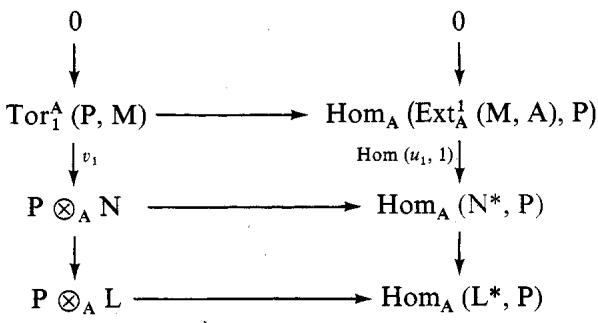
\includegraphics[keepaspectratio]{images/part001_66a54857.jpg}}

其中各列是正合的；在这种情况下我们推出结论。若 \(n \geqslant 2\) ，映射 \(u_n\) 与 \(v_n\) 是双射的（X，第 128 页，推论 4 及第 131 页，推论 3）。由归纳假设，典范同态

\[
\operatorname{Tor} _ {n - 1} ^ {\mathbf {A}} (\mathrm{P}, \mathrm{N}) \rightarrow \operatorname{Hom} _ {\mathbf {A}} \left(\operatorname{Ext} _ {\mathbf {A}} ^ {n - 1} (\mathrm{N}, \mathrm{A}), \mathrm{P}\right)
\]

是单射（相应地，双射）；图表（5）表明典范同态 \(\mathrm{Tor}_{n}^{\mathrm{A}}(\mathrm{P},\mathrm{M})\to \mathrm{Hom}_{\mathrm{A}}(\mathrm{Ext}_{\mathrm{A}}^{n}(\mathrm{M},\mathrm{A}),\mathrm{P})\) 也具有同样的性质，这完成了证明。

\subsection{环的同调维数}

定义 2. --- 称 A 的同调维数，并记作 dh(A)，其为 \(\overline{\mathbf{Z}}\) 中整数 \(n\) （存在两个 A-模 M 与 N 满足 \(\operatorname{Ext}_{\mathbf{A}}^{n}(\mathbf{M},\mathbf{N})\neq0\) ）所成集合的上确界 .

我们有 \(\mathrm{dh}(0) = -\infty\) , \(\mathrm{dh(A)} \geqslant 0\) （如果 \(A \neq 0\) ）。下面将看到 \(\mathrm{dh(A)} = 1\) （如果 \(A\) 是主理想环且不是域），并且，若 \(K\) 是一个交换域

\[
\mathrm{dh} (\mathrm{K} [ \mathrm{X} _ {1}, \dots , \mathrm{X} _ {n} ]) = n.
\]

命题 4. --- 设 n 为整数且 n ≥ 0。以下条件等价：(i) dh(A) ≤ n，

\begin{enumerate}
\def\labelenumi{(\roman{enumi})}
\setcounter{enumi}{1}
\tightlist
\item
  对每个 A-模 M，有 \(\mathrm{dp}_{\mathbf{A}}(\mathbf{M}) \leqslant n\) ,
\end{enumerate}

(ii') 对每个有限生成的 A-模 M，有 \(\mathrm{dp}_{\mathbf{A}}(\mathbf{M}) \leqslant n\) ,

\begin{enumerate}
\def\labelenumi{(\roman{enumi})}
\setcounter{enumi}{2}
\tightlist
\item
  对每个正合序列
\end{enumerate}

\[
0 \rightarrow \mathrm{K} \rightarrow \mathrm{P} _ {n - 1} \rightarrow \mathrm{P} _ {n - 2} \rightarrow \dots \rightarrow \mathrm{P} _ {0}
\]

其中 \(P_{i}\) 是投射的，K 是投射的，

\begin{enumerate}
\def\labelenumi{(\roman{enumi})}
\setcounter{enumi}{3}
\tightlist
\item
  对每个正合序列
\end{enumerate}

\[
\mathrm{I} ^ {0} \rightarrow \mathrm{I} ^ {1} \rightarrow \dots \rightarrow \mathrm{I} ^ {n - 1} \rightarrow \mathrm{N} \rightarrow 0
\]

其中 \(\mathrm{I}^{i}\) 都是内射的，N 是内射的，

\begin{enumerate}
\def\labelenumi{(\alph{enumi})}
\setcounter{enumi}{21}
\tightlist
\item
  每个 A-模都有长度不超过 n 的内射分解。
\end{enumerate}

条件 (i)、(ii) 和 (iii) 的等价性由命题 1 得出。我们显然有 (ii) \(\Rightarrow\) (ii')。因此，我们只需证明 (ii') \(\Rightarrow\) (iv) \(\Rightarrow\) (v) \(\Rightarrow\) (i)。

(ii') \(\Rightarrow\) (iv)：使用(iv)中的记号，设 K 为 \(\mathrm{I}^{0} \to \mathrm{I}^{1}\) 的核。根据 X，第 128 页，推论 4，对每个 A-模 M，我们有一个同构 \(\operatorname{Ext}_{\mathbf{A}}^{1}(\mathbf{M}, \mathbf{N}) \to \operatorname{Ext}_{\mathbf{A}}^{n+1}(\mathbf{M}, \mathbf{K})\) ；于是由(ii')可知，对每个有限生成的 A-模 M， \(\operatorname{Ext}_{\mathbf{A}}^{1}(\mathbf{M}, \mathbf{N})\) 都为零。根据 X，第 93 页，命题 11，这意味着 N 是内射的，从而得到(iv)。

\begin{enumerate}
\def\labelenumi{(\roman{enumi})}
\setcounter{enumi}{3}
\tightlist
\item
  \(\Rightarrow\) (v)：设 M 为一个 A-模。将(iv)应用于正合序列
\end{enumerate}

\[
0 \rightarrow \mathrm{M} \rightarrow \mathrm{I} ^ {0} (\mathrm{M}) \rightarrow \mathrm{I} ^ {1} (\mathrm{M}) \rightarrow \dots \rightarrow \mathrm{I} ^ {n - 1} (\mathrm{M}) \rightarrow \mathrm{K} ^ {n - 1} (\mathrm{M}) \rightarrow 0
\]

由 X，第 52 页，我们得出结论： \(\mathbf{K}^{n-1}(\mathbf{M})\) 是内射的，由此得 (v)。

\begin{enumerate}
\def\labelenumi{(\alph{enumi})}
\setcounter{enumi}{21}
\tightlist
\item
  \(\Rightarrow\) (i)：这由 X，第 100 页，定理 1 得出。
\end{enumerate}

注记. --- 1) 如果 \(\mathrm{dh}(\mathbf{A}) \leqslant n < +\infty\) ，则对每个 A-模 M 和每个右 A-模 P 有 \(\operatorname{Tor}_{n+1}^{\mathbf{A}}(\mathbf{P}, \mathbf{M}) = 0\) ，因为 \(\mathrm{dp}_{\mathbf{A}}(\mathbf{M}) \leqslant n\) （参见引理 1）。

\begin{enumerate}
\def\labelenumi{\arabic{enumi})}
\setcounter{enumi}{1}
\tightlist
\item
  为使 dh(A) 有限，必要且充分的是对每个非零 A-模 M，dp\_A(M) 均为有限。这确实由前述内容及 X，第 135 页，推论 1 得出。
\end{enumerate}

推论. --- 设 A 为左诺特环，并设 n 为整数 \textgreater{} 0. 以下条件等价：

\begin{enumerate}
\def\labelenumi{(\roman{enumi})}
\item
  \(\mathrm{dh(A)}\leqslant n,\)
\item
  对于每一对有限生成的 A-模 M 和 N，我们有 \(\operatorname{Ext}_{\mathbf{A}}^{n+1}(\mathbf{M}, \mathbf{N}) = 0\) ,
\item
  对每个有限生成的左 A-模 M 和每个有限生成的右 A-模 P，我们有 \(\operatorname{Tor}_{n+1}^{\mathbf{A}}(\mathbf{P},\mathbf{M}) = 0\) .
\end{enumerate}

这由命题 2 和 4 得出。

注记. --- 由(i)与(iii)的等价性，若 A 是右且左诺特的，则 dh(A) = dh(A°)。此等式在一般情况下不成立（X，第 204 页，习题 20）。

命题 5. --- 设 A 是左诺特的且具有有限同调维数，并令 \(\mathcal{C}_{0}\) (相应地， \(\mathcal{C}\) ) 为有限生成投射 A-模（相应地，有限生成 A-模）的同构类集合。则 Grothendieck 群的典范同态 \(\mathrm{K}(\mathcal{C}_{0}) \to \mathrm{K}(\mathcal{C})\) 是双射。

这由 X，第 137 页，推论得出。

\subsection{同调维数为0的环}

命题 6. --- 以下条件等价：

\begin{enumerate}
\def\labelenumi{(\roman{enumi})}
\item
  每个 A-模都是投射的，
\item
  每个 A-模都是内射的，
\item
  A 的每个理想都是内射模，
\item
  \(\mathrm{dh}(\mathbf{A})\leqslant 0,\)
\item
  A 是半单的，
\item
  A 是诺特的且每个 A-模都是平坦的，
\item
  每个 A-模复形都是分裂的，
\item
  每个 A-模正合列都是分裂的。
\end{enumerate}

由命题 4，我们有(i) \(\Leftrightarrow\) (ii) \(\Leftrightarrow\) (iv)；由命题 4 的推论 1，我们有(vi) \(\Rightarrow\) (iv)。由 X，第 35 页，例 4，我们有(i) \(\Rightarrow\) (vii)；由于(ii) \(\Rightarrow\) (iii)和(vii) \(\Rightarrow\) (viii)是平凡的，且由于(viii) \(\Rightarrow\) (i)由 II，第 39 页，命题 4 得出，因此只需证明(iii) \(\Rightarrow\) (v)和(v) \(\Rightarrow\) (vi)；最后一个断言由 VIII，第 5 节，第 1 号，命题 1 和 2 得出；最后，如果 A 的每个理想都是内射的，则它是 A 中的直和项，从而(iii) \(\Rightarrow\) (v)。

\subsection{同调维数为1的环}

命题 7. --- 下列条件是等价的：

\begin{enumerate}
\def\labelenumi{(\roman{enumi})}
\item
  \(\mathrm{dh}(\mathbf{A})\leqslant 1\)
\item
  投射模的每个子模都是投射的，
\end{enumerate}

(ii') A 的每个理想都是投射的，

\begin{enumerate}
\def\labelenumi{(\roman{enumi})}
\setcounter{enumi}{2}
\item
  内射 A-模的每个商都是内射的，
\item
  对每个投射复形 C，存在一个拟同构 \(\varphi : \mathbf{C} \to \mathbf{H}(\mathbf{C})\) 使得 \(\mathbf{H}(\varphi) = 1_{\mathbf{H}(\mathbf{C})}\) ,
\item
  对每个内射复形 C，存在一个拟同构 \(\psi : \mathrm{H}(\mathbf{C}) \to \mathbf{C}\) 使得 \(\mathrm{H}(\psi) = 1_{\mathrm{H}(\mathbf{C})}\) .
\item
  (i) \(\Leftrightarrow\) (ii) \(\Leftrightarrow\) (iii)：这由 X，第 138 页，命题 4 得出。
\item
  \(\Rightarrow\) (iv)：设 C 为投射复形。若(ii)成立，则 C 的子模 B(C) 是投射的，从而由 X，第 35 页，注 b) 得(iv)。
\item
  \(\Rightarrow\) (v)：设 C 为内射复形。若(iii)成立，则商 \(B_{n}(C)\) （\(C_{n+1}\) 的）对每个 \(n\) 都是内射的，从而由 X，第 35 页，注 a) 得(v)。
\item
  \(\Rightarrow\) (ii)：设 P 为投射 A-模，M 为 P 的子模， \(i: \mathbf{M} \to \mathbf{P}\) 为典范单射。设 \(p: \mathbf{L} \to \mathbf{M}\) 为自由模 L 到 M 上的满同态。考虑投射复形 C，使得 \(\mathbf{C}_1 = \mathbf{L}\) , \(\mathbf{C}_0 = \mathbf{P}\) , \(\mathbf{C}_i = 0\) （当 \(i \neq 0\) , \(1\)）， \(d_1 = i \circ p\) . 若(iv)满足，设 \(\varphi: \mathbf{C} \to \mathbf{H}(\mathbf{C})\) 为拟同构使得 \(\mathbf{H}(\varphi) = 1_{\mathbf{H}(\mathbf{C})}\) 。由于 \(\mathbf{H}_1(\mathbf{C}) = \operatorname{Ker} p\) , \(\varphi_1\) 是 L 到 \(\operatorname{Ker} p\) 上的投影算子，正合序列
\end{enumerate}

\[
0 \rightarrow \operatorname{Ker} p \rightarrow \mathrm{L} \xrightarrow {p} \mathrm{M} \rightarrow 0
\]

是分裂的，且 M 同构于 L 的一个直和项，因此是投射的。

\begin{enumerate}
\def\labelenumi{(\alph{enumi})}
\setcounter{enumi}{21}
\tightlist
\item
  \(\Rightarrow\) (iii)：设 I 为内射模，M 为 I 的商， \(\pi : \mathrm{I} \to \mathrm{M}\) 为典范投影。设 \(i: \mathrm{M} \to \mathrm{J}\) 为 M 到内射模 J 内的单同态。考虑内射复形 C，使得 \(C^0 = I\) , \(C^1 = J\) , \(C^i = 0\) （当 \(i \neq 0, 1\)）， \(d^0 = i \circ \pi\) 。若(v)满足，设 \(\psi : \mathrm{H}(\mathbf{C}) \to \mathbf{C}\) 为拟同构使得 \(\mathrm{H}(\psi) = 1_{\mathrm{H}(\mathbf{C})}\) 。由于
\end{enumerate}

\[
\mathrm{H} ^ {1} (\mathrm{C}) = \text { Coker } i  ,
\]

\(\psi^{1}\) 是典范投影 J → Coker i 的一个截面，且 M 是 J 的一个直和项，因此是内射的。

\begin{enumerate}
\def\labelenumi{(\roman{enumi})}
\setcounter{enumi}{1}
\tightlist
\item
  \(\Rightarrow\) (ii')：这是平凡的。
\end{enumerate}

(ii') \(\Rightarrow\) (ii)：这由 VII，第 3 节，定理 1 的推论 1 得出。

例. --- 若 A 是主理想环，则 dh(A) ≤ 1。

注. --- 若 A 是（交换）整环，则前述条件也等价于：

满足这些条件的整环称为戴德金环（参见 X，第 204 页，习题 12 以及 AC，VII，第 2 节，第 2 号，定理 1）。

推论. --- 设 A 为同调维数 ≤ 1 的环，C 为投射 A-模的复形， \(\tilde{C}\) 为投射右 A-模的复形，C' 为内射 A-模的复形，P 为右 A-模，M 为左 A-模，n 为整数。则我们有分裂正合序列

\[
\begin{array}{r l} & 0 \to \bigoplus_ {p + q = n} \mathrm{H} _ {p} (\tilde {\mathrm{C}}) \otimes_ {\mathrm{A}} \mathrm{H} _ {q} (\mathrm{C}) \xrightarrow {\gamma} \mathrm{H} _ {n} (\tilde {\mathrm{C}} \otimes_ {\mathrm{A}} \mathrm{C}) \xrightarrow {\alpha} \bigoplus_ {p + q = n - 1} \mathrm{Tor} _ {1} ^ {\mathrm{A}} \left(\mathrm{H} _ {p} (\tilde {\mathrm{C}}), \mathrm{H} _ {q} (\mathrm{C})\right) \to 0, \\ & 0 \to \prod_ {p} \mathrm{Ext} _ {\mathrm{A}} ^ {1} \left(\mathrm{H} _ {p} (\mathrm{C}), \mathrm{H} ^ {n - p - 1} (\mathrm{C} ^ {\prime})\right) \xrightarrow {\beta} \mathrm{H} ^ {n} (\mathrm{Homgr} _ {\mathrm{A}} (\mathrm{C}, \mathrm{C} ^ {\prime})) \\ & \qquad \qquad \qquad \xrightarrow {\lambda_ {p}} \prod_ {p} \mathrm{Homgr} _ {\mathrm{A}} \left(\mathrm{H} _ {p} (\mathrm{C}), \mathrm{H} ^ {n - p} (\mathrm{C} ^ {\prime})\right) \to 0, \\ & 0 \to \mathrm{P} \otimes_ {\mathrm{A}} \mathrm{H} _ {n} (\mathrm{C}) \xrightarrow {\gamma_ {p}} \mathrm{H} _ {n} (\mathrm{P} \otimes_ {\mathrm{A}} \mathrm{C}) \xrightarrow {\alpha_ {p}} \mathrm{Tor} _ {1} ^ {\mathrm{A}} \left(\mathrm{P}, \mathrm{H} _ {n - 1} (\mathrm{C})\right) \to 0, \\ & 0 \to \mathrm{Ext} _ {\mathrm{A}} ^ {1} \left(\mathrm{H} _ {n - 1} (\mathrm{C}), \mathrm{M}\right) \xrightarrow {\beta_ {p}} \mathrm{H} ^ {n} (\mathrm{Homgr} _ {\mathrm{A}} (\mathrm{C}, \mathrm{M})) \xrightarrow {\lambda_ {p}} \mathrm{Hom} _ {\mathrm{A}} \left(\mathrm{H} _ {n} (\mathrm{C}), \mathrm{M}\right) \to 0. \end{array}
\]

由于 \(Z(C)\) , \(B(C)\) , \(Z(\tilde{C})\) 与 \(B(\tilde{C})\) 是投射的且 \(B(C')\) 是内射的，这由 \(X\) ，第 78 页，推论 2，第 96 页，推论 1 和第 98 页，推论 2 得出。

\subsection{多项式环的同调维数}

引理 2. --- 设 \(\rho: \mathbf{A} \to \mathbf{A}'\) 为环同态，M 为 A-模， \(\mathbf{M}'\) 为 \(\mathbf{A}'\) -模。若 A-模 \(\mathbf{A}_d'\) 是平坦的，则我们有 \(\mathrm{dp}_{\mathbf{A}'}(\mathbf{A}' \otimes_{\mathbf{A}} \mathbf{M}) \leqslant \mathrm{dp}_{\mathbf{A}}(\mathbf{M})\) 。若 A-模 \(\mathbf{A}_s'\) 是投射的，则我们有 \(\mathrm{dp}_{\mathbf{A}}(\mathbf{M}') \leqslant \mathrm{dp}_{\mathbf{A}'}(\mathbf{M}')\) .

第一个断言在 \(\mathrm{dp}_{\mathbf{A}}(\mathbf{M}) = \pm \infty\) 时是显然的；若 \(\mathrm{dp}_{\mathbf{A}}(\mathbf{M}) = n \in \mathbb{N}\) ，则存在 A-模的正合序列

\[
0 \rightarrow \mathrm{P} _ {n} \rightarrow \mathrm{P} _ {n - 1} \rightarrow \dots \rightarrow \mathrm{P} _ {0} \rightarrow \mathrm{M} \rightarrow 0
\]

其中 \(P_{i}\) 是投射的；A'-模的序列

\[
0 \rightarrow \mathrm{A} ^ {\prime} \otimes_ {\mathrm{A}} \mathrm{P} _ {n} \rightarrow \mathrm{A} ^ {\prime} \otimes_ {\mathrm{A}} \mathrm{P} _ {n - 1} \rightarrow \dots \rightarrow \mathrm{A} ^ {\prime} \otimes_ {\mathrm{A}} \mathrm{P} _ {0} \rightarrow \mathrm{A} ^ {\prime} \otimes_ {\mathrm{A}} \mathrm{M} \rightarrow 0
\]

是正合的，因为 \(\mathbf{A}_d'\) 是平坦的，且 \(\mathbf{A}'\) -模 \(\mathbf{A}' \otimes_{\mathbf{A}} \mathrm{P}_i\) 是投射的（II，第 89 页，推论）；因此 \(\mathrm{dp}_{\mathbf{A}'}(\mathbf{A}' \otimes_{\mathbf{A}} \mathbf{M}) \leqslant n = \mathrm{dp}_{\mathbf{A}}(\mathbf{M})\) 。第二个断言在 \(\mathrm{dp}_{\mathbf{A}'}(\mathbf{M}') = \pm \infty\) 时是显然的；若 \(\mathrm{dp}_{\mathbf{A}'}(\mathbf{M}') = m \in \mathbf{N}\) ，则存在 \(\mathbf{A}'\) -模的一个正合序列

\[
0 \to \mathrm{P} _ {m} ^ {\prime} \to \mathrm{P} _ {m - 1} ^ {\prime} \to \dots \to \mathrm{P} _ {0} ^ {\prime} \to \mathrm{M} ^ {\prime} \to 0,
\]

其中 \(P_{i}^{\prime}\) 是投射的；底层的 A-模序列是正合的。另一方面，每个 \(P_{i}^{\prime}\) 是某个模 \(A_{s}^{\prime(I)}\) 的 A'-子模的一个直和项，因此是投射的 A-模；所以我们有 \(\mathrm{dp}_{\mathbf{A}}(\mathbf{M}^{\prime}) \leqslant m = \mathrm{dp}_{\mathbf{A}^{\prime}}(\mathbf{M}^{\prime})\) .

引理 3. --- 设 A 是交换的，并令 M 为一个 A{[}X{]}-模。

\begin{enumerate}
\def\labelenumi{\alph{enumi})}
\item
  我们有 \(\mathrm{dp}_{\mathbf{A}}(\mathbf{M}) \leqslant \mathrm{dp}_{\mathbf{A}[\mathbf{X}]}(\mathbf{M}) \leqslant \mathrm{dp}_{\mathbf{A}}(\mathbf{M}) + 1\) .
\item
  如果位似 \(X_{M}\) 是单射的，我们有 dp \(_{A}\) (M/XM) ≤ dp \(_{A[X]}\) (M)。
\item
  若 \(\mathbf{XM} = 0\) ，我们有 \(\mathrm{dp}_{\mathbf{A}}(\mathbf{M}) + 1 = \mathrm{dp}_{\mathbf{A}[\mathbf{X}]}(\mathbf{M}).\)
\item
  我们有一个 A{[}X{]}-模的正合序列（III，第 106 页及 VII，第 5 节，第 1 号）
\end{enumerate}

\[
0 \rightarrow \mathrm{A} [ \mathrm{X} ] \otimes_ {\mathrm{A}} \mathrm{M} \rightarrow \mathrm{A} [ \mathrm{X} ] \otimes_ {\mathrm{A}} \mathrm{M} \rightarrow \mathrm{M} \rightarrow 0;
\]

断言 (a) 由 X，第 135 页，推论 2 及引理 2 得出。

\begin{enumerate}
\def\labelenumi{\alph{enumi})}
\setcounter{enumi}{1}
\tightlist
\item
  若 \(\mathrm{dp}_{\mathbf{A}[\mathbf{X}]}(\mathbf{M}) = \pm \infty\) 该断言是平凡的。如果 \(\mathbf{M}\) 是投射的且非零，则 A-模 \(\mathbf{M} / \mathbf{XM}\) 等同于 \(\mathbf{A} \otimes_{\mathbf{A}[\mathbf{X}]} \mathbf{M}\) ，因此是投射的，并且我们有 \(\mathrm{dp}_{\mathbf{A}}(\mathbf{M} / \mathbf{XM}) \leqslant 0 = \mathrm{dp}_{\mathbf{A}[\mathbf{X}]}(\mathbf{M})\) 。让我们对 \(\mathrm{dp}_{\mathbf{A}[\mathbf{X}]}(\mathbf{M}) = n\) （假设其 \(>0\) ）进行归纳推理。考虑 \(\mathbf{A}[\mathbf{X}]\) -模的一个正合序列 \(0 \to \mathbf{N} \to \mathbf{L} \to \mathbf{M} \to 0\) ，其中 \(\mathbf{L}\) 是一个自由 \(\mathbf{A}[\mathbf{X}]\) -模；将该图表应用于
\end{enumerate}

\[
\begin{array}{c} 0 \longrightarrow \mathrm{N} \longrightarrow \mathrm{L} \longrightarrow \mathrm{M} \longrightarrow 0 \\ \mathrm {X_ {N}} \Big \downarrow \quad \mathrm {X_ {L}} \Big \downarrow \quad \mathrm {X_ {M}} \Big \downarrow \\ 0 \longrightarrow \mathrm{N} \longrightarrow \mathrm{L} \longrightarrow \mathrm{M} \longrightarrow 0 \end{array}
\]

将 X，第 4 页的命题 2 应用于该图表，我们看到 \(X_{N}\) 是单射的，并且我们有正合序列

\[
0 \rightarrow \mathrm{N} / \mathrm{XN} \rightarrow \mathrm{L} / \mathrm{XL} \rightarrow \mathrm{M} / \mathrm{XM} \rightarrow 0.
\]

由于 L 在 A{[}X{]} 上是自由的，L/XL 在 A 上是自由的，且我们有

\[
\mathrm{dp} _ {\mathbf {A} [ \mathbf {X} ]} (\mathbf {N}) = n - 1, \quad \mathrm{dp} _ {\mathbf {A}} (\mathbf {M} / \mathbf {X M}) \leqslant 1 + \mathrm{dp} _ {\mathbf {A}} (\mathbf {N} / \mathbf {X N});
\]

由于由归纳假设 dp \(_{A}\) (N/XN) ≤ n - 1 ，我们推出 dp \(_{A}\) (M/XM) ≤ n，这正是所要证明的。

\begin{enumerate}
\def\labelenumi{\alph{enumi})}
\setcounter{enumi}{2}
\tightlist
\item
  该断言在 \(\mathrm{dp}_{\mathbf{A}[\mathbf{X}]}(\mathbf{M}) = \pm \infty\) 时是平凡的，并且在 \(\mathrm{dp}_{\mathbf{A}[\mathbf{X}]}(\mathbf{M}) = 0\) 时也是平凡的（这是不可能的，因为 \(\mathbf{XM} = 0\) ）。因此我们可以假设 \(\mathrm{dp}_{\mathbf{A}[\mathbf{X}]}(\mathbf{M}) = n > 0\) 。如上考虑一个正合序列 \(0 \to \mathbf{N} \to \mathbf{L} \to \mathbf{M} \to 0\) ，其中 \(\mathbf{L}\) 是一个自由 \(\mathbf{A}[\mathbf{X}]\) -模，我们得到 \(\mathbf{A}\) -模的一个正合序列
\end{enumerate}

\[
0 \rightarrow \mathrm{M} \rightarrow \mathrm{N} / \mathrm{XN} \rightarrow \mathrm{L} / \mathrm{XL} \rightarrow \mathrm{M} \rightarrow 0.
\]

由 b)，我们有 \(\mathrm{dp}_{\mathbf{A}}(\mathbf{N} / \mathbf{X}\mathbf{N}) \leqslant \mathrm{dp}_{\mathbf{A}[\mathbf{X}]}(\mathbf{N}) = \mathrm{dp}_{\mathbf{A}[\mathbf{X}]}(\mathbf{M}) - 1 = n - 1\) ；由于 \(\mathrm{dp}_{\mathbf{A}}(\mathbf{L} / \mathbf{XL}) = 0\) ，从前面的正合序列出发，应用 X，第 135 页，推论 2 两次，我们推出 \(\mathrm{dp}_{\mathbf{A}}(\mathbf{M}) \leqslant n - 1\) 。但由 a)，我们有

\[
\mathrm{dp} _ {\mathbf {A}} (\mathbf {M}) \geqslant \mathrm{dp} _ {\mathbf {A} [ \mathbf {X} ]} (\mathbf {M}) - 1 = n - 1,
\]

由此得 c)。

定理 1. --- 设 A 是交换的。则

\[
\mathrm{dh} (\mathbf {A} [ \mathbf {X} ]) = \mathrm{dh} (\mathbf {A}) + 1.
\]

对每个 A{[}X{]}-模 M，我们有（引理 3）

\[
\mathrm{dp} _ {\mathbf {A} [ \mathbf {X} ]} (\mathbf {M}) \leqslant \mathrm{dp} _ {\mathbf {A}} (\mathbf {M}) + 1 \leqslant \mathrm{dh} (\mathbf {A}) + 1
\]

因此 \(\mathrm{dh}(\mathbf{A}[\mathbf{X}]) \leqslant \mathrm{dh}(\mathbf{A}) + 1\) ；反之，若 \(\mathbf{M}\) 是一个 A-模，令 \(\overline{\mathbf{M}}\) 为 \(\mathbf{A}[\mathbf{X}]\) -模，它由赋予 \(\mathbf{M}\) 使 \(\mathbf{X}\mathbf{M} = 0\) 的结构而得到，则（引理 3）

\[
\mathrm{d} p _ {\mathrm{A}} (\mathrm{M}) = \mathrm{d} p _ {\mathrm{A} [ \mathrm{X} ]} (\overline {{\mathrm{M}}}) - 1 \leqslant \mathrm{d} h (\mathrm{A} [ \mathrm{X} ]) - 1,
\]

因此 dh(A) ≤ dh(A{[}X{]}) - 1.

推论 1. --- 设 A 是交换的。我们有

\[
\mathrm{dh} (\mathrm{A} [ \mathrm{X} _ {1}, \dots , \mathrm{X} _ {n} ]) = \mathrm{dh} (\mathrm{A}) + n.
\]

这由定理对 n 进行归纳得出。

推论 2. --- 设 K 是一个交换域（相应地，一个主理想环* 或一个非域的戴德金环*）。则 dh(K{[}X₁, \ldots, Xₙ{]}) 等于 n（相应地，n + 1）。这由 dh(K) = 0（相应地，dh(K) = 1）这一事实得出。

\subsection{分次模的同调维数}

在本节中，我们假设 A 是次数 ≥ 0 的分次环。我们用 \((\mathbf{A}_{n})_{n \in \mathbf{Z}}\) 表示其分次结构；因此我们有 \(A_{n} = 0\) （对 n \textless{} 0）， \(A_{0}\) 是 A 的一个子环， \(J_{0} = \bigoplus_{n > 0} A_{n}\) 是 A 的一个双边理想，并且商分次环 \(A/J_{0}\) 等同于 \(A_{0}\) .

引理 4. --- 设 M 是一个下有界的分次 A-模（X，第 56 页）。如果 \(\mathbf{A}_0\otimes_{\mathbf{A}}\mathbf{M} = 0\) ，则 \(\mathbf{M} = 0\) .

由于 \(A_{0} \otimes_{A} M\) 同构于 \(M/J_{0} M\) ，这正是 II，第 171 页，命题 6。

引理 5. --- 设 M 是一个下有界的分次 A-模，并设

\[
s: \mathbf {A} \otimes_ {\mathbf {A} _ {0}} \mathrm{M} / \mathrm{J} _ {0} \mathrm{M} \rightarrow \mathrm{M}
\]

是一个分次 A-同态，使得 \(1 \otimes_{\mathbf{A}} s: \mathbf{A}_0 \otimes_{\mathbf{A}} (\mathbf{A} \otimes_{\mathbf{A}_0} \mathbf{M} / \mathrm{J}_0 \mathbf{M}) \to \mathbf{A}_0 \otimes_{\mathbf{A}} \mathbf{M}\) 是典范同构。则 s 是满射。若 \(\operatorname{Tor}_1^{\mathbf{A}}(\mathbf{A}_0, \mathbf{M}) = 0\) ，则 s 是双射。

我们有一个正合序列

\[
0 \rightarrow \operatorname{Ker} s \rightarrow A \otimes_ {A _ {0}} M / J _ {0} M \xrightarrow {s} M \rightarrow \operatorname{Coker} s \rightarrow 0
\]

且分次 A-模 Ker \(s\) 和 Coker \(s\) 是下有界的。由正合序列 \(\mathbf{A}_{0} \otimes_{\mathbf{A}} (\mathbf{A} \otimes_{\mathbf{A}_{0}} \mathrm{M} / \mathrm{J}_{0} \mathrm{M}) \xrightarrow{1 \otimes s} \mathbf{A}_{0} \otimes_{\mathbf{A}} \mathrm{M} \to \mathbf{A}_{0} \otimes_{\mathbf{A}} \text{Coker } s \to 0\) ，我们推出 \(\mathbf{A}_{0} \otimes_{\mathbf{A}} \text{Coker } s = 0\) ，因此 \(s\) 是满射（引理 4）。于是我们有一个正合序列

\[
\operatorname{Tor} _ {1} ^ {\mathrm{A}} \left(\mathrm{A} _ {0}, \mathrm{M}\right)\rightarrow \mathrm{A} _ {0} \otimes_ {\mathrm{A}} \operatorname{Ker} s \rightarrow \mathrm{A} _ {0} \otimes_ {\mathrm{A}} \left(\mathrm{A} \otimes_ {\mathrm{A} _ {0}} \mathrm{M} / \mathrm{J} _ {0} \mathrm{M}\right) \xrightarrow {1 \otimes s} \mathrm{A} _ {0} \otimes_ {\mathrm{A}} \mathrm{M}.
\]

若 \(\operatorname{Tor}_1^{\mathbf{A}}(\mathbf{A}_0, \mathbf{M}) = 0\) ，则 \(\mathbf{A}_0 \otimes_{\mathbf{A}} \operatorname{Ker} s = 0\) 且 \(s\) 是单射（引理 4）。

命题 8. --- 设 M 是一个下有界的分次 A-模。

\begin{enumerate}
\def\labelenumi{\alph{enumi})}
\tightlist
\item
  以下条件是等价的：
\end{enumerate}

\begin{enumerate}
\def\labelenumi{(\roman{enumi})}
\item
  M 同构于如下形式的分次 A-模： \(\mathbf{A} \otimes_{\mathbf{A}_0} \mathbf{N}\) ，其中 \(N\) 是分次投射（相应地，分次自由） \(\mathbf{A}_0\) -模；
\item
  M 是投射（相应地，自由）分次 A-模；
\item
  \(\mathbf{M} / \mathbf{J}_0\mathbf{M}\) 是投射（相应地，分次自由） \(\mathbf{A}_0\) -模，且 \(\operatorname{Tor}_1^{\mathbf{A}}(\mathbf{A}_0,\mathbf{M}) = 0\) .
\end{enumerate}

\begin{enumerate}
\def\labelenumi{\alph{enumi})}
\setcounter{enumi}{1}
\tightlist
\item
  进一步假设 M 有一个由有界次数的齐次元素组成的生成系。则以下条件等价：
\end{enumerate}

\begin{enumerate}
\def\labelenumi{(\roman{enumi})}
\item
  分次 A-模 M 具有一个有限合成列，其商同构于形如 \(A \otimes_{A_{0}} N\) 的分次 A-模，其中 N 是一个平坦分次 \(A_{0}\) -模；
\item
  M 是一个平坦 A-模；
\item
  \(\mathbf{M} / \mathrm{J}_0\mathbf{M}\) 是平坦 \(\mathbf{A}_0\) -模，且 \(\operatorname{Tor}_1^{\mathbf{A}}(\mathbf{A}_0,\mathbf{M}) = 0\) .
\end{enumerate}

在这两种情形中，我们显然有 (i) \(\Rightarrow\) (ii) \(\Rightarrow\) (iii). 因此我们必须证明 (iii) \(\Rightarrow\) (i).

\begin{enumerate}
\def\labelenumi{\alph{enumi})}
\tightlist
\item
  分次 A-模 A \(\otimes_{\mathbf{A}_0}\mathbf{M} / \mathbf{J}_0\) M 是投射 A-模，因为 \(\mathbf{M} / \mathbf{J}_0\) M 是投射 \(\mathbf{A}_0\) -模。A-模的典范同态
\end{enumerate}

\[
p: \mathbf {M} \rightarrow \mathbf {M} / \mathrm{J} _ {0} \mathbf {M}
\]

是满射；因此存在一个次数为 0 的分次 A-同态

\[
s: \mathbf {A} \otimes_ {\mathbf {A} _ {0}} \mathbf {M} / \mathrm{J} _ {0} \mathbf {M} \rightarrow \mathbf {M}
\]

使得 \(p \circ s(a \otimes x) = ax\) （对 \(a \in A\) 和 \(x \in M / J_0 M\) ）.

根据引理 5， \(s\) 是从 \(\mathbf{A} \otimes_{\mathbf{A}_0} \mathrm{M} / \mathrm{J}_0 \mathrm{M}\) 到 \(\mathbf{M}\) 上的 A-模同构，由此得 (i)。

\begin{enumerate}
\def\labelenumi{\alph{enumi})}
\setcounter{enumi}{1}
\tightlist
\item
  根据对 M 的假设，存在整数 a, b 使得 \(a \leqslant b\) 且 M 由 \(\oplus M_{i}\) 生成。让我们对正整数 b - a 进行归纳推理。
\end{enumerate}

若 \(b - a = 0\) 则 M 由 \(\mathbf{M}_a\) 生成，且典范 \(\mathbf{A}_0\) -同态 \(\mathbf{M}_a \to \mathbf{M} / \mathbf{J}_0\) M 是双射的；于是由 A-同态 \(\mathbf{A} \otimes_{\mathbf{A}_0} \mathbf{M}_a \to \mathbf{M}\) （由 M 作为 A-模的结构所定义）可推出一个分次 A-同态

\[
s: \mathbf {A} \otimes_ {\mathbf {A} _ {0}} \mathbf {M} / \mathrm{J} _ {0} \mathbf {M} \rightarrow \mathbf {M}
\]

满足引理 5 的条件。于是由引理 5，s 是双射的，从而 (i) 成立。

在一般情形中，设 \(\mathbf{M}^{(a)}\) 为 M 的由 \(M_{a}\) 生成的（分次）子 A-模，且设 \(M'\) 为商 \(\mathbf{M}/\mathbf{M}^{(a)}\) 。我们有一个正合序列

\[
0 \to \mathbf {M} ^ {(a)} \xrightarrow {f} \mathbf {M} \xrightarrow {g} \mathbf {M} ^ {\prime} \to 0,
\]

由此，由于根据假设 \(\mathrm{Tor}_{1}^{\mathbf{A}}(\mathbf{A}_{0},\mathbf{M}) = 0\) ，有正合序列

\begin{enumerate}
\def\labelenumi{(\arabic{enumi})}
\setcounter{enumi}{5}
\tightlist
\item
\end{enumerate}

\[
\begin{array}{c} \operatorname{Tor} _ {2} ^ {\mathsf {A}} (\mathbf {A} _ {0}, \mathbf {M} ^ {\prime}) \to \operatorname{Tor} _ {1} ^ {\mathsf {A}} (\mathbf {A} _ {0}, \mathbf {M} ^ {(a)}) \to 0 \\ 0 \to \operatorname{Tor} _ {1} ^ {\mathsf {A}} (\mathbf {A} _ {0}, \mathbf {M} ^ {\prime}) \to \operatorname{M} ^ {(a)} / \mathrm{J} _ {0} \operatorname{M} ^ {(a)} \xrightarrow {1 \otimes f} \operatorname{M} / \mathrm{J} _ {0} \operatorname{M} \xrightarrow {1 \otimes g} \operatorname{M} ^ {\prime} / \mathrm{J} _ {0} \operatorname{M} ^ {\prime} \to 0. \end{array}\tag{7}
\]

但典范同态 \(M_{a} \to M^{(a)}/J_{0} M^{(a)}\) 是双射的。由此可知同态 \(1 \otimes f : M^{(a)}/J_{0} M^{(a)} \to M/J_{0} M\) 是单射的，并且其像是 \(A_{0}\) -子模的、 \(M/J_{0} M\) 的一个直和项。由此，从正合序列 (7) 可得 \(\operatorname{Tor}_{1}^{A}(A_{0}, M') = 0\) ，且 \(A_{0}\) -模 \(M'/J_{0} M'\) 是平坦的，因为它同构于 \(M/J_{0} M\) 的一个直和项。根据归纳假设（该假设适用于 \(M'\) ，因为后者由 \(M'^{i}\) （\(a < i \leqslant b\) ）所生成）， \(M'\) 满足条件 (i)，因此是平坦的。于是从正合序列 (6) 可推出 \(\operatorname{Tor}_{1}^{A}(A_{0}, M^{(a)}) = 0\) ，而 \(M^{(a)}/J_{0} M^{(a)}\) 等同于 \(M_{a}\) ，后者是一个平坦的 \(A_{0}\) -模（作为 \(M/J_{0} M\) 的一个直和项子模）；根据已经证明的结果，分次 A-模 \(M^{(a)}\) 同构于 \(A \otimes_{A_{0}} M_{a}\) ，因此也满足 (i)，这完成了证明。

推论 1. --- 设 M 是一个有限生成的分次 A-模。如果 \(\mathbf{A}_0\) -模 \(\mathrm{M} / \mathrm{J}_0\) M 是投射的（相应地，分次自由的，相应地，平坦的），并且如果 \(\operatorname{Tor}_1^{\mathbf{A}}(\mathbf{A}_0, \mathbf{M}) = 0\) 则 A-模 M 是投射的（相应地，分次自由的，相应地，平坦的）。

推论 2. --- 假设每个投射 \(\mathbf{A}_{0}\) -模是自由的（相应地，设 A 是诺特的，且每个有限生成的投射 \(\mathbf{A}_{0}\) -模是自由的）。设 M 是一个下有界的分次 A-模（相应地，一个有限生成的分次 A-模），并设 n 为一个整数 \(\geqslant 0\) 使得 \(\mathrm{dp}_{\mathbf{A}}(\mathbf{M}) \leqslant n\) 。存在一个由分次 A-模与次数为 0 的分次同态构成的正合序列

\[
0 \rightarrow \mathrm{L} _ {n} \rightarrow \mathrm{L} _ {n - 1} \rightarrow \dots \rightarrow \mathrm{L} _ {0} \rightarrow \mathrm{M} \rightarrow 0
\]

其中 \(L_{i}\) 是分次自由的且有下界（相应地，分次自由且有限生成）。

事实上，存在（X，第 56 页，命题 11）一个由分次 A-模与 0 次同态构成的正合序列

\[
0 \to \mathrm{L} _ {n} \to \mathrm{L} _ {n - 1} \to \dots \to \mathrm{L} _ {0} \to \mathrm{M} \to 0
\]

其中 \(L_{i}\) 对 \(0 \leqslant i \leqslant n\) 是下方有界的（相应地，有限生成的），且对 \(0 \leqslant i \leqslant n - 1\) 是分次自由的 .

由于 \(\mathrm{dp}_{\mathbf{A}}(\mathbf{M}) \leqslant n\) ，A-模 \(L_{n}\) 是投射的；因此 \(\mathbf{A}_0 \otimes_{\mathbf{A}} L_n\) 是一个投射 \(\mathbf{A}_0\) -模，从而是分次自由的；由于 \(L_{n}\) 在下方有界且 \(\mathbf{A}_0 \otimes_{\mathbf{A}} L_n\) 分次自由， \(L_{n}\) 是分次自由的（命题 7）。

推论 3（希尔伯特合冲定理）. --- 假设 \(\mathbf{A}_0\) 是一个交换域，且 A 作为 \(\mathbf{A}_0\) -代数由 \(n\) 个次数 \(>0\) 的代数无关齐次元素生成。对于每个下方有界（相应地，有限型）的分次 A-模 M，存在一个由分次 A-模和次数为 0 的分次同态构成的正合序列

\[
0 \rightarrow L _ {n} \rightarrow L _ {n - 1} \rightarrow \dots \rightarrow L _ {0} \rightarrow M \rightarrow 0,
\]

其中 \(L_{i}\) 是分次自由的且有下界（相应地，且有限生成）。

事实上，由 X，第 143 页，定理 1 有 \(\mathrm{dh}(\mathbf{A}) = n\) ，并应用推论 2。

注记. --- 推论 2 也适用于以下情形：

\begin{enumerate}
\def\labelenumi{\alph{enumi})}
\item
  \(\mathbf{A}_0\) 是主理想环且 \(\mathbf{A} = \mathbf{A}_0[\mathbf{X}_1, \dots, \mathbf{X}_{n-1}]\) ;
\item
  * A \(_{0}\) 是维数为 r 的正则局部诺特环，且 A = A \(_{0}\) {[}X \(_{1}\) , \ldots，X \(_{n}\) ，r{]}. *
\end{enumerate}

推论 4. --- 假设 \(\mathbf{A}_{0}\) 半单。设 M 为有下界的分次 A-模，n 为整数 \(\geqslant 0\) 。对于 \(\mathrm{dp}_{\mathbf{A}}(\mathbf{M}) \leqslant n\) ，其充要条件是 \(\operatorname{Tor}_{n+1}^{\mathbf{A}}(\mathbf{A}_{0}, \mathbf{M}) = 0\) .

若 \(\mathrm{dp}_{\mathbf{A}}(\mathbf{M}) \leqslant n\) ，则 \(\operatorname{Tor}_{n+1}^{\mathbf{A}}(\mathbf{A}_0, \mathbf{M}) = 0\) （X，第 135 页，引理 1）。反之，设 \(0 \to \mathbf{K} \to \mathbf{L}_{n-1} \to \ldots \to \mathbf{L}_1 \to \mathbf{L}_0 \to \mathbf{M} \to 0\) 是下方有界的分次 A-模的正合序列，使得 \(\mathbf{L}_0, \ldots, \mathbf{L}_{n-1}\) 是分次自由的（X，第 56 页，命题 11）；由 X 第 131 页的推论 3，等式 \(\operatorname{Tor}_{n+1}^{\mathbf{A}}(\mathbf{A}_0, \mathbf{M}) = 0\) 蕴含 \(\operatorname{Tor}_1^{\mathbf{A}}(\mathbf{A}_0, \mathbf{K}) = 0\) ；由于 \(\mathbf{K} / \mathbf{J}_0\mathbf{K}\) 是一个投射 \(\mathbf{A}_0\) -模（因为 \(\mathbf{A}_0\) 是半单的；X，第 140 页，命题 6），K 由命题 8（X，第 144 页）是投射的，且 \(\mathrm{dp}_{\mathbf{A}}(\mathbf{M}) \leqslant n\) .

推论 5. --- 设环 \(\mathbf{A}_0\) 半单。若 \(\operatorname{Tor}_{n+1}^{\mathbf{A}}(\mathbf{A}_0, \mathbf{A}_0) = 0\) ，则我们有 \(\mathrm{dp}_{\mathbf{A}}(\mathbf{M}) \leqslant n\) （对每个下方有界的分次 \(\mathbf{A}\) -模）。

设 A° 表示 A 的反分次环：我们有 (A°)₀ = (A₀)°，因此 (A°)₀ 是半单的（VIII，§ 5，n° 1，注记 3）。由于 \(\operatorname{Tor}_{n+1}^{A°}(A₀°, A₀°) = 0\) ，由推论 4 有 \(\mathrm{dp}_A(A₀s) \leqslant n\) ：这意味着对每个 A-模 M 有 \(\operatorname{Tor}_{n+1}^{A°}(M₀, A₀°) = 0\) ，因此 \(\operatorname{Tor}_{n+1}^{A}(A₀, M) = 0\) ，我们应用推论 4。

\section{科斯居尔复形}

在本段中，所考虑的所有环都是交换环。
